% -*- coding: utf-8 -*-

\begin{chapter}{Тепловой баланс океана}\label{chap:5}
% \chapter{The Oceanic Heat Budget}
Примерно половина солнечной энергии, достигающей Земли, поглощается океаном
и сушей, где она затем временно сохраняется вблизи поверхности, и лишь 
около~$20\%$~--- непосредственно 
атмосферой. Большая часть энергии, поглощенной некоторым участком океана, 
возвращается обратно в атмосферу над этим же участком благодаря испарению
и инфракрасному излучению с его поверхности. Остальная же переносится 
течениями в другие области, в особенности в средние широты. 
%% "особенно" или в "частности", происходит в средних широтах или туда перенос?
%
% About half the solar energy reaching earth is absorbed by the ocean and land, 
% where it is temporarily stored near the surface. Only about a fifth of the 
% available solar energy is directly absorbed by the atmosphere. Of the energy 
% absorbed by the ocean, most is released locally to the atmosphere, mostly 
% by evaporation and infrared radiation. The remainder is transported 
% \index{transport!heat}by currents to other areas especially mid latitudes. 

Теплоотдача океана в тропиках~--- основной источник тепла, требуемого для
поддержания атмосферной циркуляции. Кроме того, запас тепла, который создается
в океане летом, позволяет сгладить изменения погодных условий зимой.
%% ??? "климат", вроде, это погода, усредненная за 30 лет???
Перенос тепла океанскими течениями непостоянен, так что существенные изменения
в этом процессе, в частности, в Атлантическом океане, могли играть 
значительную роль в развитии ледниковых периодов. Как следствие, изучение
теплового баланса океанов и процессов переноса тепла занимают важное место
в изучении земного климата и его краткосрочной и долгосрочной изменчивости.
%
% Heat lost by the tropical ocean is the major source of heat needed to drive 
% the atmospheric circulation. And, solar energy stored in the ocean from summer 
% to winter helps ameliorate earth's climate. The thermal energy transported 
% by ocean currents is not steady, and significant changes in the transport,
% particularly in the Atlantic, may have been important for the development 
% of the ice ages. For these reasons, oceanic heat budgets and transports 
% are important for understanding earth's climate and its short and long term 
% variability.

\begin{section}{Тепловой баланс океана}
% \section{The Oceanic Heat Budget}
Изменение количества энергии, запасенной верхними слоями океана, происходит
благодаря дисбалансу между притоком и оттоком тепла через морскую 
поверхность. Перенос тепла через эту поверхность называется 
\emph{потоком тепла}. Потоки тепла и воды оказывают влияние на плотность
поверхностных вод и, следовательно, на их плавучесть. Благодаря этому,
суммарный поток тепла и воды часто принято называть \emph{потоком плавучести}.
%
% \index{heat budget|textbf}Changes in energy stored in the upper ocean result
% from an imbalance between input and output of heat through the sea surface.
% This transfer of heat across or through a surface is called a
% \textit{heat flux}\index{heat flux|textbf}. The flux of heat and water also
% changes the density of surface waters, and hence their buoyancy. As a result,
% the sum of the heat and water fluxes is often called the 
% \textit{buoyancy flux}\index{buoyancy flux|textbf}\index{flux!buoyancy}.

Поток энергии в глубинные слои океана обычно гораздо слабее, чем поток через
поверхность. В то же время, результирующий поток энергии, входящей в океан 
и исходящей из него, должен быть нулевым: в противном случае, океан бы либо 
разогревался, либо, наоборот, охлаждался. Сумма потоков тепла, входящих в
некоторый объем воды либо исходящих из него, называется 
\emph{тепловым балансом}.
%
% The flux of energy to deeper layers is usually much smaller than the flux 
% through the surface. And, the total flux of energy into and out of the ocean 
% must be zero, otherwise the ocean as a whole would heat up or cool down. 
% The sum of the heat fluxes into or out of a volume of water is 
% the \textit{heat budget}.\index{heat budget!terms of}

Основные слагаемые теплового баланса на поверхности океана таковы:
%
% The major terms in the budget at the sea surface are:
\begin{enumerate}
\item
\emph{Инсоляция}~$Q_{SW}$~--- поток солнечной энергии, поглощаемой океаном.
%% "поглощаемой" ли?
%
% \vitem \textit{Insolation} $Q_{SW}$, \index{insolation|textbf}the flux of 
% solar energy into the sea; 

\item
\emph{Суммарная инфракрасная радиация}~$Q_{LW}$~--- суммарный поток излучения
инфракрасной радиации от поверхности океана.
%
% \vitem \textit{Net Infrared Radiation} $Q_{LW}$, 
% \index{net infrared radiation|textbf}net flux of infrared radiation from 
% the sea;

\item
\emph{Поток явного тепла}~$Q_S$~--- исходящий поток тепла, возникающий 
за счет теплопроводности (кондуктивный теплообмен).
%
% \vitem \textit{Sensible Heat Flux} $Q_S$, 
% \index{sensible heat flux|textbf}the flux of heat out of the sea due 
% to conduction; 

\item
\emph{Поток скрытого тепла}~$Q_L$~--- поток энергии, переносимой вместе с
водяными парами.
%
% \vitem \textit{Latent Heat Flux}
% $Q_L$, \index{latent heat flux|textbf}the flux of energy carried by evaporated 
% water; and 

\item
\emph{Адвекция}~$Q_V$~--- горизонтальный перенос тепла течениями.
%
% \vitem \textit{Advection} $Q_V$, \index{advection|textbf}heat carried away by
% currents.
\end{enumerate}

Согласно закону сохранения тепла,
%
% Conservation of heat requires:
%
\begin{equation}
Q = Q_{SW} + Q_{LW} + Q_S + Q_L + Q_V,
\end{equation}
где~$Q$~--- результирующий приток или отток тепла. Единицей измерения потоков 
тепла служит~$\wpsqm$. Произведение потока тепла на площадь водной поверхности 
и на время дает количество энергии, выраженное в джоулях. Изменение температуры 
воды~$\Delta t$ зависит от изменения энергии по закону
\begin{equation}
\Delta E = C_{p} \, m \, \Delta t,
\end{equation}
где~$m$~--- масса охлаждаемой/нагреваемой воды, а~$C_p$~--- удельная 
теплоемкость воды при постоянном давлении:
\begin{equation}\label{eq:Cpwater}
C_{p} \approx 4.0\times 10^{3} 
 \mbox{~$\mbox{Дж} \cdot \mbox{кг}^{-1} \cdot \vphantom{1}^\circ \mbox{C}^{-1}$}.
\end{equation}
Так, для нагрева~$1\kg$ морской воды на~$\degCent{1}$ 
потребуется $4\,000\Joules$~энергии (рис.~\ref{fig:Cp}).
%
% where $Q$ is the resultant heat gain or loss. Units for heat 
% fluxes\index{heat flux!units of} are watts/m$^2$. The product of flux times 
% surface area times time is energy in joules. The change in temperature 
% $\Delta t$ of the water is related to change in energy $\Delta E$ through:
% \begin{equation}
% \Delta E = C_{p} \, m \, \Delta t
% \end{equation}
% where $m$ is the mass of water being warmed or cooled, and $C_p$ is the 
% specific heat of sea water at constant pressure.
% \begin{equation}
% C_{p} \approx 4.0\times 10^{3} \mbox{ J}\cdot \mbox{kg}^{-1} \cdot \, ^\circ
% \mbox{C}^{-1}
% \end{equation}
% Thus, 4,000 joules of energy are required to heat 1.0 kilogram of sea water by
% 1.0$^{\circ}$C (figure 5.1).

\begin{figure}[t!]
\includegraphics{pics/Cp}
\caption{Удельная теплоемкость~$C_{p}$ морской воды при атмосферном давлении
в~$\text{Дж} \cdot \text{кг} / {}^\circ \text{C}$ как функция 
температуры по шкале Цельсия и солености, вычисленная по эмпирической 
формуле Millero et al. (1973), используя алгоритмы Fofonoff and Millard (1983). 
Нижняя линия соответствует точке замерзания морской воды.}
\label{fig:Cp}
\end{figure}
%
% \begin{figure}[t!]
% \includegraphics{Cp}
% \footnotesize Figure 5.1 Specific heat of \rule{0pt}{3ex}sea water at
% atmospheric pressure
% $C_{p}$ in joules per gram per degree Celsius as a function of temperature in
% Celsius and salinity, calculated from the empirical formula given by Millero
% et al. (1973) using algorithms in Fofonoff and Millard (1983). The
% lower line is the freezing point of salt water.
% \label{fig:Cp}
% \vspace{-3ex}
% \end{figure}

\begin{paragraph}{Важность роли океана в тепловом балансе Земли.}
% \paragraph{Importance of the Ocean in Earth's Heat Budget}
Чтобы понять, насколько важен вклад океана в тепловой баланс Земли в целом,
сравним количество тепла, накапливающегося в океане и на суше в течение года.
В рамках этого периода, тепло накапливается летом и рассеивается зимой.
Наша цель~--- показать, что океан в этих процессах существенно опережает сушу.
%
% \index{heat budget!importance of}To understand the importance of
% the ocean in earth's heat budget, let's make a comparison
% of the heat stored in the ocean with heat stored on land during an
% annual cycle. During the cycle, heat is stored in summer and
% released in the winter. The point is to show that the ocean store
% and release much more heat than the land.

Для начала, сравним удельные теплоемкости воды~(\ref{eq:Cpwater}), почвы 
и скальных пород:
%% одна теплоемкость на двоих?
\begin{equation}
C_{p(\text{скал})} = 800 
 \mbox{~$\mbox{Дж}\cdot \mbox{кг}^{-1} \cdot \vphantom{1}^\circ \mbox{C}^{-1}$,}
\end{equation}
откуда получим, что~$C_{p(\text{скал})} \approx 0.2 \, C_{p(\text{воды})}$.
%
% To begin, use (5.3) and the heat capacity of soil and rocks
% \begin{equation}
% C_{p(rock)} = 800 \mbox{ J}\cdot \mbox{kg}^{-1} \cdot \, ^\circ \mbox{C}^{-1}
% \end{equation}
% to obtain $C_{p(rock)} \approx 0.2 \, C_{p(water)}$.

Объем воды, вовлеченной в теплообмен с атмосферой в течение годового цикла,
составляет~$100\cubm$ на $1\sqm$~поверхности, то есть, поверхностный водный 
слой толщиной~$100\m$. Принимая во внимание плотность воды, 
равную~$1000\kgpcm$, легко вычислить массу воды, находящейся под воздействием 
атмосферы: $\mbox{плотность}\times\mbox{объем} = 100\,000\kg$. Аналогичный
объем для суши составляет~$1\cubm$, плотность скальных пород~--- $3\,000\kgpcm$,
а масса~--- $3\,000\kg$ соответственно. 
%
% The volume of water which exchanges heat with the atmosphere on a seasonal cycle
% is 100 m$^3$ per square meter of surface, i.e. that mass from the surface to a
% depth of 100 meters. The density of water is 1000 kg/m$^3$, and the mass in
% contact with the atmosphere is density $\times$ volume = $m_{water} = 100,000$
% kg. The volume of land which exchanges heat with the atmosphere on a seasonal
% cycle is 1 m$^3$. Because the density of rock is 3,000 kg/m$^3$, the mass of the
% soil and rock in contact with the atmosphere is 3,000 kg.

Используя эти величины, легко посчитать поглощение тепла океаном и сушей:
\begin{align*}
\Delta E_{\text{океана}} & = C_{p(\text{воды})} \, m_{\text{воды}}\, \Delta t && \Delta t = \degCent{10} \\
                         & = (4000) (10^5) (10)\Joules \\
                         & = 4.0 \times 10^9\Joules \\
\Delta E_{\text{суши}}   & = C_{p(\text{скал})} \, m_{\text{скал}}\, \Delta t & & \Delta t = \degCent{20} \\
                         & = (800) (3000) (20)\Joules \\
                         & = 4.8 \times 10^7\Joules \\
\frac{\Delta E_{\text{океана}}}{\Delta E_{\text{суши}}}  & = 100
\end{align*}
где $\Delta t$~--- типичная разница летней и зимней температур.
%
% The seasonal heat storage\index{heat storage!seasonal} values for the ocean 
% and land are therefore:
% \begin{align}
% \Delta E_{ocean} & = C_{p(water)} \, m_{water}\, \Delta t && \Delta t = 10^{\circ} \text{C} \notag \\
%                  & = (4000) (10^5) (10^{\circ}) \text{Joules}       \notag  \\
%                  & = 4.0 \times 10^9 \, \text{Joules}                 \notag  \\
% \Delta E_{land}  & = C_{p(rock)} \, m_{rock}\, \Delta t & & \Delta t = 20^{\circ} \text{C} \notag \\
%                  & = (800) (3000) (20^{\circ}) \text{Joules}        \notag  \\
%                  & = 4.8 \times 10^7 \, \text{Joules}               \notag  \\
% \frac{\Delta E_{ocean}}{\Delta E_{land}}  & = 100 \notag
% \end{align}
% where $\Delta t$ is the typical change in temperature from summer to winter.

Такое существенное различие в количестве тепла, запасенного океаном и сушей,
имеет важные последствия. Годовой диапазон температур воздуха возрастает по
мере удаления от океана и может превысить~$\degrees{40}$ в центре континентов,
а в Сибири достигает даже~$\degrees{60}$. В то же время, колебания температуры
воздуха над океаном и вдоль побережья не превышают~$\degCent{10}$, а 
изменчивость температуры воды еще более низка (рис.~\ref{fig:SSTvariability}, 
внизу).
%
% The large storage of heat in the ocean compared with the land has important
% consequences. The seasonal range of air temperatures on land increases with
% distance from the ocean, and it can exceed 40\degrees C in the center of
% continents, reaching 60\degrees C in Siberia. Typical range of temperature over
% the ocean and along coasts is less than 10\degrees C. The variability of water
% temperatures is still smaller (see figure 6.3, bottom).
\end{paragraph}
\end{section}

\begin{section}{Слагаемые теплового баланса}
%\section{Heat-Budget Terms}
Рассмотрим подробнее факторы, влияющие на каждое слагаемое теплового баланса.
%
%\index{heat budget!terms of}Let's look at the factors influencing
%each term in the heat budget.

\begin{paragraph}{Факторы, влияющие на инсоляцию.}
% \paragraph{Factors Influencing Insolation}
Количество входящей солнечной радиации определяется, в основном, широтой,
временем года, временем суток и облачностью. Так, полярные регионы нагреваются
слабее тропиков, а нагрев одних и те же регионов различается зимой и летом,
ранним утром и в полдень, в облачный и ясный день соответственно.
%
% \index{insolation!factors influencing}Incoming solar radiation is primarily 
% determined by latitude, season, time of day, and cloudiness. The polar
% regions are heated less than the tropics, areas in winter are
% heated less than the same area in summer, areas in early morning
% are heated less than the same area at noon, and cloudy days have
% less sun than sunny days.

Факторы, которые следует учитывать, таковы:
%
%The following factors are important:
\begin{enumerate}
\item
Высота Солнца над горизонтом, которая зависит от широты, времени года 
и времени суток. Не следует забывать, что ночью инсоляция отсутствует!
%
% \vitem
% The height of the sun\index{sun!height above horizon} above the horizon, 
% which depends on latitude, season, and time of day. Don't forget, there 
% is no insolation\index{insolation} at night!

\item
Продолжительность светового дня, зависящая от широты и времени года.
%
% \vitem
% The length of day, which depends on latitude and season.

\item
Площадь сечения поверхности, поглощающей солнечный свет, определяемая высотой
%% почему именно "cross-sectional area",  "площадь сечения"?
Солнца над горизонтом.
%
% \vitem
% The cross-sectional area of the surface absorbing sunlight, which depends on
% height of the sun above the horizon.

\item
Потери солнечной радиации в атмосфере, которые зависят от:
\begin{enumerate}
   \item облачного покрова, который поглощает и рассеивает излучение; 
   \item длины пути луча сквозь атмосферу, изменяющейся 
         пропорционально~$\csc \varphi$, где~$\varphi$~--- угловая
         высота Солнца над горизонтом ;
   \item поглощения молекулами газов солнечного излучения в определенных 
         диапазонах (рис.~\ref{fig:insolation}); при этом играет роль 
         концентрация различных
         газов: $\text{H}_2\text{O}$, $\text{O}_3$, $\text{CO}_2$;
   \item поглощения и рассеивания солнечной радиации аэрозолями 
         как морского, так и вулканического происходжения;
   \item наличия в атмосфере пыли, рассеивающей излучение, в особенности
         пыли из пустыни Сахара над Атлантическим океаном.
\end{enumerate}
%
% \vitem
% Attenuation, which depends on: i) Clouds, which absorb and scatter
% radiation. ii) Path length through the atmosphere, which varies as
% $\csc \varphi$, where $\varphi$ is angle of the sun above the
% horizon. iii) Gas molecules which absorb radiation in some bands
% (figure 5.2). H$_2$O, O$_3$, and CO$_2$ are all important. iv)
% Aerosols which scatter and absorb radiation. Both volcanic and marine
% aerosols are important. And v) dust, which scatters radiation,
% especially Saharan dust over the Atlantic.

\item
Отражающей способности поверхности, определяемой высотой Солнца над горизонтом
и гладкостью морской поверхности.
%
% \vitem
% Reflectivity of the surface, which depends on solar elevation angle and roughness
% of sea surface.
\end{enumerate}
Среди этих факторов преобладает влияние высоты Солнца над горизонтом и 
облачности. Поглощение солнечной радиации озоном, водяными парами, аэрозолями
и пылью гораздо слабее.
% 
% Solar inclination and cloudiness dominate. Absorption by ozone, water
% vapor, aerosols, and dust are much weaker.

\begin{figure}[t!]
\makebox [121 mm][c]{\includegraphics{pics/insolation}}
\caption{Инсоляция (спектральная освещенность) солнечного света на верхней
границе атмосферы и на поверхности моря при ясной погоде. Штриховая линия
отображает сглаженную кривую излучения абсолютно черного тела, размер и
расстояние до которого соответствуют Солнцу. Обозначив число масс атмосферы
как~$m$, получаем, что $m = 2$ соответствует высоте Солнца над горизонтом
около~$\degrees{30}$ (Stewart, 1985: 43).}
\label{fig:insolation}
\end{figure}
%
% \begin{figure}[t!]
% \makebox [121 mm] [c] {\includegraphics{insolation}}
% \footnotesize
% Figure 5.2 Insolation\index{insolation!at top of atmosphere} \rule{0pt}{3ex}
% (spectral irradiance) of sunlight at top of the atmosphere and at the sea 
% surface on a clear day. The dashed line is the best-fitting curve of 
% blackbody radiation the size and distance of the sun. The number of standard 
% atmospheric masses is designated by $m$. Thus $m = 2$ is applicable for 
% sunlight when the sun\index{sun!height above horizon} is 30\degrees above the
% horizon. After Stewart (1985: 43).
% \label{fig:insolation}
% \vspace{-3ex}
% \end{figure}

\begin{figure}[t!]
\includegraphics{pics/QswDown}
\caption{Среднемесячные величины потока солнечной радиации через безоблачную
атмосферу в океан в течение~1989~г., вычисленные в Центре анализа спутниковых 
данных (Исследовательский центр НАСА, Лэнгли) на основе данных Международного 
проекта по спутниковой климатологии (Darnell et al. 1992).}
\label{fig:QswDown}
\end{figure}
%
% \begin{figure}[t!]
% \includegraphics{QswDown}
% \footnotesize
% Figure 5.3 Monthly average of \rule{0pt}{3ex}downward flux of sunlight through 
% a cloud-free sky and into the ocean in W/m$^2$ during 1989 calculated 
% by the Satellite Data Analysis Center at the \textsc{nasa} Langley Research 
% Center (Darnell et al. 1992) using data from the International Satellite 
% Cloud Climatology Project.
% \label{fig:QswDown}
% \vspace{-3ex}
% \end{figure}

Величина среднегодовой инсоляции (рис.~\ref{fig:QswDown}) находится в диапазоне
%
% The average annual value for insolation\index{insolation!annual average} 
% (figure 5.3) is in the range:
\begin{equation}
30\wpsqm < Q_{SW} < 260\wpsqm.
\end{equation}
\end{paragraph}

\begin{paragraph}{Факторы, влияющие на исходящий поток инфракрасной радиации.}
% \paragraph{Factors Influencing Infrared Flux}
Излучение морской поверхности равно излучению абсолютно черного тела, имеющего
температуру, равную температуре воды, что составляет приблизительно~$290\Kelv$.
Распределение излучения как функции длины волны определяется уравнением Планка.
Морская вода при температуре~$290\Kelv$ излучает сильнее всего в диапазоне
около~$10\mum$. Волны такой длины активно поглощаются облаками и, в некоторой
степени, водяными парами. График атмосферной проницаемости как функции длины
волны в атмосфере без загрязнений, но с различной концентрацией водяных паров,
представлен на рис.~\ref{fig:transmittance}. Он показывает, что в некоторых 
диапазонах длин волн, называемых окнами, атмосфера практически прозрачна.
%
% \index{infrared flux!factors influencing}The sea surface radiates as 
% a blackbody having the same temperature as the water, which is roughly 290 K. 
% The distribution of radiation as a function of wavelength is given by Planck's 
% equation. Sea water at 290 K radiates most strongly at wavelengths near 
% 10 $\mu$m. These wavelengths are strongly absorbed by clouds, and somewhat 
% by water vapor. A plot of atmospheric transmittance as a function of wavelength 
% for a clear atmosphere but with varying amounts of water vapor (figure 5.4) 
% shows the atmosphere is nearly transparent in some wavelength bands called 
% windows.

\begin{figure}[t!]
\makebox [121 mm][c]{\includegraphics{pics/transmittance}}
\caption{Проницаемость атмосферы в вертикальном направлении от границы с 
космическим пространством до морской поверхности для шести моделей атмосферы
с очень хорошей ($23\km$) видимостью, учитывающих молекулярное и аэрозольное
рассеивание.  Отметим влияние водяного пара на проницаемость атмосферы 
в окне~$10$--$14\mum$, что, в свою очередь, определяет поток~$Q_{LW}$, 
достигающий максимума в этом диапазоне Selby and McClatchey (1975).}
\label{fig:transmittance}
\end{figure}
%
% \begin{figure}[t!]
% \makebox [121 mm] [c] {\includegraphics{transmittance}}
% \footnotesize
% Figure 5.4 Atmospheric 
% \rule{0pt}{3ex}transmittance\index{atmospheric transmittance} for a 
% vertical path to space from sea level for six model atmospheres with very 
% clear, 23 \textit{km}, visibility, including the influence of molecular 
% and aerosol scattering. Notice how water vapor modulates the transparency 
% of the 10-14 $\mu$m atmospheric window, hence it modulates $Q_{LW}$, which 
% is a maximum at these wavelengths. After Selby and McClatchey (1975).
% \label{fig:transmittance}
% \vspace{-3ex}
% \end{figure}

Проницаемость атмосферы в диапазоне~$8$--$13\mum$ в безоблачный день
определяется, в основном, концентрацией водяных паров. Поглощение в других
диапазонах, например, $3.5$--$4.0\mum$, зависит от 
концентрации~$\text{CO}_2$. С её ростом окно исчезает, и доля излучения,
поглощаемого атмосферой, увеличивается.
%
% The transmittance on a cloud-free day through the window from 8 $\mu$m to 13
% $\mu$m is determined mostly by water vapor. Absorption in other bands, such as
% those at 3.5 $\mu$m to 4.0 $\mu$m depends on CO$_2$ concentration in the 
% atmosphere. As the concentration of CO$_2$ increases, these windows close 
% and more radiation is trapped by the atmosphere.

Благодаря тому, что атмосфера в целом прозрачна для входящего солнечного
излучения и в определенной мере непрозрачна для исходящей инфракрасной
радиации, в ней задерживается некоторая энергия. Этот запас энергии в 
сочетании с атмосферной конвекцией поддерживают температуру земной 
поверхности на $\degrees{33}$~выше, чем та, которая бы установилась 
в результате достижения температурного баланса с космосом при отсутствии 
влажной атмосферы с протекающими в ней процессами конвекции. 
Атмосфера влияет на теплообмен подобно стеклянным стенам теплицы, благодаря 
чему эффект повышения температуры поверхности получил название 
\emph{парникового эффекта}. Обсуждение радиационного баланса планеты в 
достаточно простом изложении доступно в работе Hartmann (1994: 24--26).
В механизме парникового эффекта важную роль играют так называемые 
парниковые газы: $\text{CO}_2$, водяные пары, метан и озон.
%
% Because the atmosphere is mostly transparent to incoming sunlight, and
% somewhat opaque to outgoing infrared radiation, the atmosphere traps
% radiation.  The trapped radiation, coupled with convection in the
% atmosphere, keeps earth's surface 33\degrees\ warmer than it would be
% in the absence of a convecting, wet atmosphere but in thermal
% equilibrium with space.  The atmosphere acts like the panes of glass
% on a greenhouse, and the effect is known as the \textit{greenhouse
% effect}\index{greenhouse effect|textbf}.  See Hartmann (1994: 24--26)
% for a simple discussion of the radiative balance of a planet. CO$_2$,
% water vapor, methane, and ozone are all important greenhouse gasses.

Суммарный поток инфракрасной радиации с поверхности океана зависит от 
следующих факторов:
%
% The net infrared flux\index{infrared flux!net} depends on:
\begin{enumerate}
\item
Толщина облаков. Чем толще облачный слой, тем меньше тепла рассеивается 
в космос.
%
% \vitem Clouds thickness. The thicker the cloud deck, the less heat
% escapes to space.

\item
Высота облачного слоя, которая определяет его температуру, а следовательно,
и количество энергии, которую облачный слой излучает обратно в океан. Эта
энергия пропорциональна~$t^4$, где~$t$~--- температура излучающего тела
в кельвинах. Чем выше расположен облачный слой, тем он холоднее.
%
% \vitem Cloud height, which determines the temperature at which the
% cloud radiates heat back to the ocean. The rate is proportional to
% $t^4$, where $t$ is the temperature of the radiating body in
% Kelvins. High clouds are colder than low clouds.

\item
Содержание водяного пара в атмосфере. Чем влажнее атмосфера, тем меньше
тепла излучается в космос.
%
% \vitem Atmospheric water-vapor content. The more humid the atmosphere
% the less heat escapes to space.

\item
Температура воды. Чем теплее вода, тем больше тепла она излучает. Как было
сказано выше, уровень излучения зависит от температуры пропорционально~$t^4$. 
%
% \vitem Water Temperature. The hotter the water the more heat is
% radiated.  Again, radiation depends of $t^4$.

\item
Величина ледяного и снежного покрова. Лед также излучает энергию подобно
абсолютно черному телу, но он охлаждается гораздо быстрее воды. Моря, покрытые
льдом, изолированы от атмосферы.
%
% \vitem Ice and snow cover. Ice emits as a black body, but it cools
% much faster than open water. Ice-covered seas are insulated from the
% atmosphere.
\end{enumerate}

Влияние количества водяных паров и облачности на суммарный отток инфракрасной
радиации превышает влияние поверхностной температуры. Более теплые тропические
регионы теряют меньше тепла, чем более холодные полярные. Диапазон изменения
температур от полюсов до экватора~--- $\degCent{0} < t < \degCent{25}$ 
или~$273\Kelv < t < 298\Kelv$, а отношение максимальной температуры в 
кельвинах к минимальной равно~$298/273 = 1.092$. Возведя его в четвертую
степень, получаем~$1.42$. Таким образом, количество излучаемой радиации
за счет изменения поверхностной температуры возрастает от полюса к экватору 
на~$42\%$. На том же самом расстоянии влияние водяных паров может 
превысить~$200\%$. 
%
% Water vapor and clouds influence the net loss of infrared radiation
% more than surface temperature. Hot tropical regions lose less heat
% than cold polar regions. The temperature range from poles to equator
% is $0^{\circ}\rm{C} < t < 25^{\circ}\rm{C}$ or $273\rm{K} < t <
% 298\rm{K}$, and the ratio of maximum to minimum temperature in Kelvins
% is 298/273 = 1.092. Raised to the fourth power this is 1.42. Thus
% there is a 42\% increase in emitted radiation from pole to
% equator. Over the same distance water vapor can change the net emitted
% radiance by 200\%.

Среднее годовое значение суммарного потока инфракрасной радиации находится
в достаточно узком диапазоне:
%
% The average annual value for net infrared 
% flux\index{infrared flux!annual average} is in the narrow range:
\begin{equation}
-60\wpsqm < Q_{LW} < -30\wpsqm.
\end{equation}
\end{paragraph}

\begin{paragraph}{Факторы, влияющие на поток скрытого тепла.}
%\paragraph{Factors Influencing Latent-Heat Flux}
Поток скрытого тепла зависит, в основном, от скорости ветра
и относительной влажности. Более сильные ветры и сухой воздух способствуют
испарению большего количества влаги, чем слабые ветры и относительная 
влажность, близкая к~$100\%$. В полярных регионах испарение с покрытой льдом
поверхности океана значительно ниже, чем с открытой воды, так что в Арктике
%% In polar regions ... . In the arctic --- в чем нюанс? 
%% Почему именно в Арктике?
океан в основном теряет тепло через разводья (участки морской поверхности, 
свободные от льда). Как следствие, доля открытой воды (\emph{ледовитость}) 
играет очень важную роль в арктическом тепловом балансе.
%
% \index{latent heat flux}Latent heat flux is influenced primarily by
% wind speed and relative humidity. High winds and dry air evaporate
% much more water than weak winds with relative humidity near 100\%. In
% polar regions, evaporation from ice covered ocean is much less than
% from open water. In the arctic, most of the heat lost from the sea is
% through leads (ice-free areas). Hence the percent open water is very
% important for the arctic heat budget.

Среднегодовое значение потока скрытого тепла лежит в таких пределах:
%
% The average annual value for latent-heat flux is in the range:
\begin{equation}
-130\wpsqm < Q_{L} < -10\wpsqm.
\end{equation}
\end{paragraph}

\begin{paragraph}{Факторы, влияющие на поток явного тепла.}
% \paragraph{Factors Influencing Sensible-Heat Flux}
Поток явного тепла определяется скоростью ветра и разницей температур воды
и воздуха. Высокая скорость ветра и большой перепад температур вызывают
больший поток. Можно сказать, что к океану в известном смысле применимо
понятие <<жёсткости погоды>>.
%
% \index{sensible heat flux}Sensible heat flux is influenced by wind
% speed and air-sea temperature difference. High winds and large
% temperature differences cause high fluxes. Think of this as a
% wind-chill factor for the ocean.

Среднегодовое значение потока явного тепла ограничено такими рамками:
%
% The average annual value for sensible-heat flux is in the range:
\begin{equation}
-42\wpsqm < Q_{S} < -2 \wpsqm.
\end{equation}
\end{paragraph}
\end{section}

\begin{section}{Прямое вычисление потоков тепла}
%\section[Direct Calculation of Fluxes]{Direct Calculation of Fluxes}
Перед тем, как описать географическое распространение потоков тепла в океан
и из него, нам следует выяснить, как эти потоки измеряются либо вычисляются.
%
% Before we can describe the geographical distribution of fluxes
% into and out of the ocean, we need to know how they are measured
% or calculated.

\begin{paragraph}{Оценка турбулентных потоков на основе измерения порывистости
ветра.}
%\paragraph{Gust-Probe Measurements of Turbulent Fluxes}
В данный момент известен единственный достаточно точный метод вычисления 
потоков скрытого и явного тепла, а также потока момента движения морской
поверхности: прямое измерение турбулентных явлений в атмосферном пограничном
слое при помощи измерителей порывистости ветра, установленных на низколетящих
самолетах или прибрежных буйковых станциях. Количество проведенных измерений
%% offshore platform ??? 
очень невелико, поскольку они дороги, а также неприменимы для вычисления 
осредненных потоков тепла в течение длительных промежутков времени либо 
на больших площадях. Данные, полученные при помощи измерителей порывистости
ветра, применяются лишь для калибровки других методов вычисления потоков.
%
% \index{flux!direct calculation of!gust probe measurement}There is only
% one accurate method for calculating fluxes of sensible and latent heat
% and momentum at the sea surface: from direct measurement of turbulent
% quantities in the atmospheric boundary layer made by gust probes on
% low-flying aircraft or offshore platforms. Very few such measurements
% have been made. They are expensive, and they cannot be used to
% calculate heat fluxes\index{heat flux!measurements of} averaged over
% many days or large areas. The gust-probe measurements are used only to
% calibrate other methods of calculating fluxes.

\begin{enumerate}
\item
Измерения следует проводить в поверхностном подслое атмосферного пограничного
слоя (разд.~\ref{sec:BoundaryLayer}), обычно на высоте до~$30\m$ над уровнем
моря, поскольку потоки в этом слое не зависят от высоты.
% 
% \vitem Measurements must be made in the surface layer of the
% atmospheric boundary layer (See \S 4.3), usually within 30 m of the
% sea surface, because fluxes are independent of height in this layer.

\item
Применяемые приборы (измерители порывистости ветра) должны иметь высокое 
быстродействие: несколько измерений в секунду для стационарных либо одно
измерение на каждый метр для установленных на самолетах.
%% каждый метр чего???
%
% \vitem Measurements must be made by fast-response instruments (gust
% probes) able to make several observations per second on a tower, or
% every meter from a plane.

\item
Измерению подлежат такие величины, как вертикальная и горизонтальная 
составляющие ветра, влажность и температура воздуха.
%
% \vitem Measurements include the horizontal and vertical components of
% the wind, the humidity, and the air temperature.
\end{enumerate}

Потоки вычисляются на основе корреляции вертикальной и горизонтальной 
составляющих ветра, влажности и температуры. Каждая разновидность потоков
требует для своего вычисления различных исходных данных ($u'$, $w'$, $t'$
и~$q'$):
%
% Fluxes are calculated from the correlation of vertical wind and
% horizontal wind, humidity, or temperature: Each type of flux is
% calculated from different measured variables, $u'$, $w'$, $t'$, and
% $q'$:
\begin{subequations}
\begin{align}
T   &= \langle \rho_a \,{u'w'}\rangle = \rho_a \, \langle {u'w'}\rangle \equiv \rho_a \,u_*^2,\\
Q_S &= C_p\,\langle\rho_a\,{w't'}\rangle = \rho_a \, {C_p} \, \langle{w't'}\rangle,\\ 
Q_L &= L_E \, \langle{w'q'}\rangle,
\end{align}
\end{subequations}
где угловые скобки обозначают осреднение по времени либо пространству, а
другие используемые обозначения приведены в табл.~\ref{tbl:5.1}. Заметим, 
что упомянутая там \emph{удельная влажность} представляет собой массу 
водяных паров, содержащихся в единичном объеме воздуха.
%
% where the brackets denotes time or space averages, and the notation is
% given in table 5.1. Note that \textit{specific
% humidity}\index{specific humidity|textbf} mentioned in the table is
% the mass of water vapor per unit mass of air.

\begin{table}
\caption{Обозначения величин, определяющих потоки}\label{tbl:5.1}
\begin{small}
\begin{tabular}{llc}
Символ & Переменная & Значение/Размерность\\
\hline
$C_p$    & Удельная теплоемкость воздуха                          & $1030\mbox{~Дж}\cdot \mbox{кг}^{-1}\cdot \mbox{К}^{-1}$ \\
$C_D$    & Коэффициент сопротивления (см.~\ref{sec:BoundaryLayer})& $(0.50 + 0.071 \, U_{10})\times 10^{-3}$                \\
%% в оригинале отсылка к разд. 4.3, но по смыслу -- к 4.6
$C_L$    & Коэффициент скрытой теплопередачи                      & $1.2 \times 10^{-3}$                                    \\
$C_S$    & Коэффициент явной теплопередачи                        & $1.0 \times 10^{-3}$                                    \\
$L_E$    & Скрытая теплота парообразования                        & $2.5 \times 10^6\mbox{~Дж/кг}$                          \\
$q$      & Удельная влажность воздуха                             & кг (вод. паров)/кг (возд.)                              \\
$q_a$    & Удельная влажность воздуха на высоте~$10\m$            & кг (вод. паров)/кг (возд.)                              \\
$q_s$    & Удельная влажность воздуха на уровне моря              & кг (вод. паров)/кг (возд.)                              \\
$Q_S$    & Поток явного тепла                                     & $\wpsqm$                                                \\
$Q_L$    & Поток скрытого тепла                                   & $\wpsqm$                                                \\
$T$      & Ветровое напряжение                                    & Па                                                      \\
$t_a$    & Температура воздуха на высоте~$10\m$                   & К или $\degCent{\vphantom{0}}$                          \\
$t_s$    & Температура морской поверхности                        & К или $\degCent{\vphantom{0}}$                          \\
$t'$     & Температурная флуктуация                               & $\degCent{\vphantom{0}}$                                \\
$u'$     & Горизонтальная составляющая флуктуации ветра           & м/с                                                     \\
$u_*$    & Скорость трения                                        & м/с                                                     \\
$U_{10}$ & Скорость ветра на высоте~$10\m$                        & м/с                                                     \\
$w'$     & Горизонтальная составляющая флуктуации ветра           & м/с                                                     \\
$\rho_a$ & Плотность воздуха                                      & $1.3\kgpcm$                                             \\
$T$      & Вектор ветрового напряжения                            & Па                                                      \\
\hline
\end{tabular}
\end{small}
$C_S$ и~$C_L$ по Smith (1988).
\end{table}
%
% \begin{table}[t!]\small
% \begin{tabular*}{121mm}{@{}llc@{}}
% \multicolumn{3}{@{}l@{}}{\bfseries Table 5.1 Notation \rule[-1ex]{0mm}{1ex}Describing Fluxes}         \\
% \hline
% Symbol   &  Variable    \rule{0mm}{2.5ex}                  & Value and Units                          \\
% \hline
% $C_p$    &  Specific heat capacity of air\rule{0mm}{2.5ex} & 1030 J$\cdot$kg$^{-1}\cdot$K$^{-1}$      \\
% $C_D$    &  Drag coefficient  (see 4.3)                    & $(0.50 + 0.071 \, U_{10})\times
% 10^{-3}$ \\
% $C_L$    &  Latent heat transfer coefficient               & $1.2 \times 10^{-3}$                     \\
% $C_S$    &  Sensible heat transfer coefficient             & $1.0 \times 10^{-3}$                     \\
% $L_E$    &  Latent heat of evaporation                     & $2.5 \times 10^6$ J/kg                   \\
% $q$      &  Specific humidity of air                       & kg (water vapor)/kg (air)                \\
% $q_a$    &  Specific humidity of air 10 m above the sea    & kg (water vapor)/kg (air)                \\
% $q_s$    &  Specific humidity of air at the sea surface    & kg (water vapor)/kg (air)                \\
% $Q_S$    &  Sensible heat flux                             & W/m$^{2}$                                \\
% $Q_L$    &  Latent heat flux                               & W/m$^{2}$                                \\
% $T$      &  Wind stress                                    & Pascals                                  \\
% $t_a$    &  Temperature of the air 10 m above the sea      & K or
% $^{\circ}$C                         \\
% $t_s$    &  Sea-surface temperature                        & K or
% $^{\circ}$C                         \\
% $t'$     &  Temperature fluctuation                        & $^{\circ}C$                              \\
% $u'$     &  Horizontal component of fluctuation of wind    & m/s                                      \\
% $u_*$    &  Friction velocity                              & m/s                                      \\
% $U_{10}$ &  Wind speed at 10 m above the sea               & m/s                                      \\
% $w'$     &  Vertical component of wind fluctuation         & m/s                                      \\
% $\rho_a$   &  Density of air                                 & 1.3 kg/m$^{3}$                           \\
% $T$      &  Vector wind stress                             &
% Pa                                       \\ [0.5ex]
% \hline
% \end{tabular*} \\ [0.5ex]
% $C_S$ and $C_L$ from Smith (1988).
% \vspace {-3ex}
% \end{table}
\end{paragraph}

\begin{paragraph}{Радиометрические измерения потоков излучения.}
%\paragraph{Radiometer Measurements of Radiative Fluxes}
Радиометры, установленные на судах, буйковых станциях и даже небольших 
островах, применяются для прямых измерений потоков излучения. Широкополосные
радиометры, чувствительные к излучению в диапазоне~$0.3$--$50\mum$,
способны измерить входящее солнечное и тепловое излучение с точностью 
порядка~$3\%$ при условии, что они были хорошо откалиброваны и тщательно
обслуживаются. Другие, специализированные, радиометры могут измерить входящее
солнечное излучение, а также входящую и исходящую инфракрасную радиацию.
%
% \index{flux!direct calculation of!radiometer measurements}Radiometers
% on ships, offshore platforms, and even small islands are used to make
% direct measurements of radiative fluxes. Wideband radiometers
% sensitive to radiation from 0.3 $\mu$m to 50 $\mu$m can measure
% incoming solar and infrared radiation with an
% accuracy\index{accuracy!fluxes!radiative} of around 3\% provided they
% are well calibrated and maintained. Other, specialized radiometers can
% measure the incoming solar radiation, the downward infrared radiation,
% and the upward infrared radiation.
\end{paragraph}
\end{section}

\begin{section}{Косвенное вычисление потоков: приближенные формулы}
% \section{Indirect Calculation of Fluxes: Bulk Formulas}
Использование датчиков порывистости ветра обходится дорого, а радиометры
требуют тщательного ухода. Ни те, ни другие не могут применяться при
получении долгосрочных глобальных величин потоков. Чтобы рассчитать 
характеристики этих потоков на основе практически осуществимых измерений,
воспользуемся установленной в ходе наблюдений корреляцией между потоками
и значением величин, которые могут быть измерены глобально.
%
% \index{flux!indirect calculation of!bulk formulas}The use of
% gust-probes is very expensive, and radiometers must be carefully
% maintained. Neither can be used to obtain long-term, global values of
% fluxes. To calculate these fluxes from practical measurements, we use
% observed correlations between fluxes and variables that can be
% measured globally.

В случае потоков явного и скрытого тепла, а также момента движения, эти
корреляции называются \emph{приближенными формулами}. 
%
% For fluxes of sensible and latent heat and momentum, the correlations
% are called \textit{bulk formulas}. \index{bulk formulas|textbf}They
% are:
\begin{subequations}
\begin{align}
T     & = \rho_a \,C_D \, U^{2}_{10} \\
Q_S   & = \rho_a \, C_p \,C_S \, U_{10} \, (t_s - t_a) \\
Q_L   & = \rho_a \,  L_E  \, C_L \, U_{10} \,(q_s - q_a) \label{eq:bulklatentheap}
\end{align}
\end{subequations}

Температура воздуха~$t_a$ измеряется термометрами, установленными на судах,
поскольку измерить ее со спутников невозможно. В то же время, 
температура~$t_s$ может быть определена как судовыми приборами, так и из 
космоса при помощи инфракрасных радиометров, таких как~AVHRR 
(Advanced Very High Resolution Radiometer).
%
% Air temperature $t_a$ is measured using thermometers on ships. It
% cannot be measured from space using satellite instruments. $t_s$ is
% measured using thermometers on ships or from space using infrared
% radiometers such as the \textsc{avhrr}\index{Advanced Very High
% Resolution Radiometer (AVHRR)}.

Удельная влажность воздуха на высоте~$10\m$ над уровнем моря~$q_a$
вычисляется на основе судовых измерений относительной влажности воздуха.
В работе~Gill (1982: pp: 39--41, 43--44, \& 605--607) приводятся уравнения,
определяющие взаимосвязь давления и плотности водяных паров с удельной
теплоемкостью влажного воздуха. Удельная влажность на уровне моря~$q_s$
вычисляется на основе~$t_s$ в предположении, что воздух, непосредственно
контактирующий с морской поверхностью, насыщен водяными парами. Скорость
ветра~$U_{10}$ измеряется либо вычисляется при помощи методов и инструментов,
описанных в гл.~\ref{chap:4}. Отметим, что ветровое напряжение представляет
собой вектор, характеризующийся модулем и направлением: параллельно морской
поверхности в направлении ветра.
%
% The specific humidity of air at 10 m above the sea surface $q_a$ is
% calculated from measurements of relative humidity made from
% ships. Gill (1982: pp: 39--41, 43--44, \& 605--607) describes
% equations relating water vapor pressure, vapor density, and specific
% heat capacity of wet air. The specific humidity at the sea surface
% $q_s$ is calculated from $t_s$ assuming the air at the surface is
% saturated with water vapor. $U_{10}$ is measured or calculated using
% the instruments or techniques described in Chapter 4. Note that wind
% stress\index{wind stress!is a vector} is a vector with magnitude and
% direction. It is parallel to the surface in the direction of the wind.

С учетом сказанного выше, задача принимает вид: как рассчитать потоки через
морскую поверхность, требуемые для изучения динамики океана? Эти потоки 
включают: напряжение, нагрев солнечным излучением, испарение, суммарный
исходящий поток инфракрасной радиации, осадки, потоки явного тепла и прочие,
такие как потоки~$\text{CO}_2$ и частиц, формирующих морские аэрозоли.
Более того, нам потребуется вычисление величин потоков с высокой точностью,
примерно, $\pm 15\wpsqm$. Это эквивалентно потоку тепла, способному нагреть
или охладить водяной столб глубиной~$100\m$ примерно на~$\degCent{1}$ в год.
В табл.~\ref{tbl:5.2} приводится типичная точность измерения различных потоков
инструментами космического базирования. Далее мы подробнее рассмотрим каждую 
переменную.
%
% The problem now becomes: How to calculate the fluxes across the sea
% surface required for studies of ocean dynamics? The fluxes include: 1)
% stress; 2) solar heating; 3) evaporation; 4) net infrared radiation;
% 5) rain; 5) sensible heat; and 6) others such as CO$_2$ and particles
% (which produce marine aerosols). Furthermore, the fluxes must be
% accurate. We need an accuracy\index{accuracy!heat fluxes} of
% approximately $\pm$15 W/m$^2$. This is equivalent to the flux of heat
% which would warm or cool a column of water 100 m deep by roughly
% 1\degrees{C} in one year. Table 5.2 lists typical accuracies of fluxes
% measured globally from space. Now, let's look at each variable.

\begin{table}
\caption{Погрешность определения характеристик ветра и потоков 
по спутниковым данным}\label{tbl:5.2}
\begin{small}
\begin{tabular}{p{0.3\textwidth}lp{0.45\textwidth}}
\hline
Переменная & Погрешность & Комментарии \\
\hline
Скорость ветра                    & $\pm 1.5\mps$        & погрешность измерения                             \\
                                  & $\pm 1.5\mps$        & погрешность выборочной оценки (среднемесячная)    \\
Ветровое напряжение               & $\pm 10\%$           & погрешность коэффициента сопротивления            \\
                                  & $\pm 14\Pa$          & при скорости ветра~$10\mps$                       \\
Инсоляция                         & $\pm 5\%$            & среднемесячная                                    \\
                                  & $\pm 15\wpsqm$       & среднемесячная                                    \\
                                  & $\pm 10\%$           & среднесуточная                                    \\
Интенсивность осадков             & $\pm 50\%$           &                                                   \\
Сумма осадков                     & $\pm 10\%$           & участок $\degrees{5} \times \degrees{5}$ для~TRMM \\
Суммарная длинноволновая радиация & $\pm 4$--$8\%$       & среднесуточная                                    \\
                                  & $\pm 15$--$27\wpsqm$ &                                                   \\
Поток скрытого тепла              & $\pm 35\wpsqm$       & среднесуточный                                    \\
                                  & $\pm 15\wpsqm$       & среднемесячный                                    \\
\hline
\end{tabular}
\end{small}
\end{table}
%
% \begin{table}[t!]\small \centering
% \begin{tabular*}{120mm}{@{}lll@{}}
% \multicolumn{3}{@{}l@{}}{\bfseries Table 5.2 Accuracy of \rule[-1ex]{0mm}{1ex}Wind
% and Fluxes Observed Globally From Space} \\
% \hline
% Variable         & Accuracy          & Comments   \rule{0mm}{2.5ex}             \\
% \hline
% Wind Speed       & $\pm$1.5 m/s      & Instrument Error\rule{0ex}{2.5ex}        \\
%                  & $\pm$1.5 m/s      & Sampling Error (Monthly Average)         \\
% Wind Stress       & $\pm$10 \%        & Drag Coefficient Error\rule{0ex}{2.5ex}  \\
%                  & $\pm$14 Pa        & Assuming 10 m/s Wind Speed               \\
% Insolation       & $\pm$5 \%         & Monthly Average\rule{0ex}{2.5ex}         \\
%                  & $\pm$15 W/m$^2$   & Monthly Average                          \\
%                  & $\pm$10 \%        & Daily Average                            \\
% Rain Rate        & $\pm$50 \%        &  \rule{0ex}{2.5ex}                       \\
% Rainfall         & $\pm$10 \%        & $5^{\circ} \times 5^{\circ}$ area for \textsc{trmm}\rule{0ex}{2.5ex} \\
% Net Long Wave Radiation & $\pm$4--8 \%  & Daily Average\rule{0ex}{2.5ex}        \\
%                         & $\pm$15--27 W/m$^2$  &                                \\
% Latent Heat Flux & $\pm$35 W/m$^2$   & Daily Average\rule{0ex}{2.5ex}           \\
%                                                                     & $\pm$15 W/m$^2$   & Monthly Average                          \\ [0.5ex]
% \hline
% \end{tabular*} \\[0.5ex]
% \vspace{-3ex}
% \end{table}

\begin{paragraph}{Скорость ветра и ветровое напряжение.}
% \paragraph{Wind Speed and Stress}
Ветровое напряжение вычисляется на основе судовых наблюдений за ветром
и данных спутниковых скаттерометров, как это было рассмотрено 
в гл.~\ref{chap:4}.
%
% \index{wind stress!calculation of}\index{wind!speed}Stress is
% calculated from wind observations made from ships at sea and from
% scatterometers\index{scatterometers}\index{wind!from scatterometers}
% in space as described in the last chapter.
\end{paragraph}

\begin{paragraph}{Инсоляция.}
% \paragraph{Insolation}
Инсоляция вычисляется на основе характеристик облачности, определенных как в
результате судовых наблюдений, так и по показаниям радиометров видимого 
диапазона, установленных на метеоспутниках. Спутниковые данные намного точнее,
поскольку измерить облачный слой, находясь под ним, крайне затруднительно.
Обработка этих данных осуществляется в рамках Международного проекта 
по спутниковой климатологии облаков (ИСККП), результаты работы которого
служат основой при составлении карт инсоляции, в том числе и ее ежемесячной 
изменчивости (Darnell et al. 1988; Rossow and Schiffer 1991).
%% ISCCP
%
% \index{insolation!calculation of} is calculated from cloud
% observations made from ships and from visible-light radiometers on
% meteorological satellites. Satellite measurements are far more
% accurate than the ship data because it's very hard to measure
% cloudiness from below the clouds. Satellite measurements processed by
% the International Satellite Cloud Climatology Project \textsc{isccp}
% are the basis for maps of insolation\index{insolation!maps of} and its
% variability from month to month (Darnell et al. 1988; Rossow and
% Schiffer 1991).

В основе метода расчета инсоляции лежит следующая идея. Величину солнечного
излучения на внешней границе атмосферы можно рассчитать, исходя из солнечной
постоянной, географических координат и времени. На своем дальнейшем пути 
в атмосфере солнечное излучение либо отражается облачным покровом обратно 
в космос, либо в конечном счете достигает земной поверхности. Доля излучения,
поглощенного атмосферой при этом невелика и почти постоянна. Однако, 
в некоторых современных работах Cess et al. (1995) and Ramanathan et al. (1995)
полнота этих соображений оспаривается в пользу гипотезы, что поглощение
в атмосфере может быть функцией облачности. Взяв за основу первоначальное 
утверждение, можно вычислить инсоляцию по следующей формуле:
$$
  \text{Инсоляция} = S (1 - A) - C,
$$
где величина~$S = 1365\wpsqm$~--- солнечная постоянная, $A$~--- альбедо
(отношение отраженного излучения к входящему), а~$C$~--- константа, включающая
поглощение солнечного излучения озоном и другими атмосферными газами, а также
облачными каплями. Вычисление инсоляции производится на основе данных о
состоянии облачного покрова (куда входит и количество излучения, отраженного
атмосферными аэрозолями), полученных с приборов, установленных на 
метеоспутниках, таких, как~AVHRR. Поглощение излучения озоном и другими газами
рассчитывается на основе данных об их распределении в атмосфере.
Точность расчета~$Q_{SW}$ по спутниковым данным составляет~5--7\%.
%
% The basic idea behind the calculation of
% insolation\index{insolation!calculation of} is this. Sunlight at the
% top of the atmosphere is accurately known from the solar
% constant\index{solar constant!and insolation}, latitude, longitude,
% and time. Sunlight is either reflected back to space by clouds, or it
% eventually reaches the sea surface. Only a small and nearly constant
% fraction is absorbed in the atmosphere. But, recent work by Cess et
% al. (1995) and Ramanathan et al. (1995) suggest that this basic idea
% may be incomplete, and that atmospheric absorption may be a function
% of cloudiness. Assuming atmospheric absorption is constant,
% insolation\index{insolation!calculation of} is calculated from:
% \[
% \text{Insolation} = S (1 - A) - C
% \]
% where $S = 1365$ W/m$^2$ is the solar constant\index{solar
% constant!value}, $A$ is albedo, the ratio of incident to reflected
% sunlight, and $C$ is a constant which includes absorption by ozone and
% other atmospheric gases and by cloud droplets. Insolation is
% calculated from cloud data (which also includes reflection from
% aerosols) collected from instruments such as the \textsc{avhrr}
% \index{Advanced Very High Resolution Radiometer (AVHRR)}on
% meteorological satellites.  Ozone and gas absorption are calculated
% from known distributions of the gases in the atmosphere. Q$_{SW}$ is
% calculated from satellite data with an
% accuracy\index{accuracy!short-wave radiation} of 5--7\%.
\end{paragraph}

\begin{paragraph}{Входящий поток воды (атмосферные осадки).}
%\paragraph{Water Flux In (Rainfall)}
Количество осадков~--- еще одна величина, которую крайне сложно измерить
приборами, установленными на судах. Показания дождемеров, установленных
в разных местах судна и на причале,
различаются более чем в два раза. Дождь в море под воздействием ветра 
падает практически горизонтально; кроме того, путь дождевых капель искажается
судовыми надстройками. Также во многих регионах дождь выпадает в виде
мороси, которую трудно обнаружить и измерить.
%
% \index{flux!water flux!calculation of}\index{water flux!calculation
% of}\index{rainfall!calculation of}Rain rate is another variable that
% is very difficult to measure from ships. Rain collected from gauges at
% different locations on ships and from gauges on nearby docks all
% differ by more than a factor of two. Rain at sea falls mostly
% horizontally because of wind, and the ship's superstructure distorts
% the paths of raindrops. Rain in many areas falls mostly as drizzle,
% and it is difficult to detect and measure.

Наиболее точно количество осадков в тропиках~($\pm \degrees{35}$)
измеряется микроволновыми радиометрами и радарными наблюдениями на различных
частотах, используя инструменты Проекта по измерению осадков в тропиках (ТРММ),
начатого в 1997~г. Количество осадков в других регионах или за другой
промежуток времени может быть достаточно точно определено по объединенным
данным о микроволновом излучении, результатам наблюдений высоты верхней 
границы облачного покрова в инфракрасном диапазоне и по показаниям 
дождемеров~(рис.~\ref{fig:precip}). Также количество осадков может быть 
рассчитано на основе реанализа погодных данных при помощи численных моделей 
атмосферной циркуляции (Schubert, Rood, and Pfaendtner, 1993), 
либо путем объединения судовых и спутниковых наблюдений с результатами 
численных моделей прогноза погоды (Xie and Arkin, 1997).
%
% The most accurate measurements of rain rate in the tropics ($\pm
% 35$\degrees) are calculated from microwave radiometers and radar
% observations of rain at several frequencies using instruments on the
% Tropical Rain Measuring Mission \textsc{trmm} launched in 1997. Rain
% for other times and latitudes can be calculated accurately by
% combining microwave data with infrared observations of the height of
% cloud tops and with rain gauge data (figure 5.5). Rain is also
% calculated from the reanalyses weather data by numerical models of the
% atmospheric circulation (Schubert, Rood, and Pfaendtner, 1993), and by
% combining ship and satellite observations with analyses from numerical
% weather-prediction models (Xie and Arkin, 1997).

Источником наиболее существенных проблем служит вычисление суммы осадков 
по их интенсивности, подверженное ошибкам выборочного обследования.
Выпадение осадков представляет собой сравнительно редкое событие, 
распределение которого подчиняется логнормальному закону; большая часть
осадков происходит из небольшого количества storms.
%% ??? storm = ливень, циклон, буря, шторм
Спутники зачастую пропускают их появление, а чтобы получить практически
%% логическая связь пропущенного шторма и необходимости осреднять???
пригодные величины суммарных осадков, данные приходится осреднять по участкам
со стороной до~$\degrees{5}$.
%% что есть "сторона участка"?
%
% The largest source of error is due to conversion of rain rate to
% cumulative rainfall\index{rainfall!cumulative}, a sampling
% error\index{sampling error}. Rain is very rare, it is log-normally
% distributed, and most rain comes from a few storms. Satellites tend to
% miss storms, and data must be averaged over areas up to 5\degrees\ on
% a side to obtain useful values of rainfall.

\begin{figure}[t!]
\includegraphics{pics/precip} 
\caption{Количество осадков (м/год), вычисленное на основе данных,
собранных в ходе Глобального проекта по климатологии осадков 
(Центр космических полетов Годдарда, НАСА)
на основе показаний дождемеров, а также данных, полученных
с инфракрасных радиометров, установленных на геосинхронных метеоспутниках,
и SSM/I. Шаг изолиний~--- $0.5\mpyr$, количество осадков в закрашенных областях
превышает~$2\mpyr$ в более светлых и~$3\mpyr$ в более темных зонах, 
соответственно.}
\label{fig:precip}
\end{figure}
%
%\begin{figure}[t!]
%\includegraphics{precip} 
%\footnotesize Figure 5.5 Rainfall\index{rainfall!map}
%\rule{0pt}{3ex}in m/year calculated \index{global
%precipitation!map of}from data compiled by the Global
%Precipitation Climatology Project at \textsc{nasa}'s Goddard Space
%Flight Center using data from rain gauges, infrared radiometers on
%geosynchronous meteorological satellites, and the \textsc{ssm/i}.
%Contour interval is 0.5 m/yr, light shaded areas exceed 2 m/yr,
%heavy shaded areas exceed 3 m/yr. \label{fig:precip}
%\vspace{-4ex}
%\end{figure}
\end{paragraph}

\begin{paragraph}{Суммарная длинноволновая радиация.}
%\paragraph{Net Long-Wave Radiation}
Суммарная длинноволновая радиация с трудом поддается вычислению, поскольку
зависит от высоты и толщины облачного слоя, а также от вертикального 
распределения водяных паров в атмосфере. Для ее расчета применяются численные
модели прогноза погоды, либо же она вычисляется на основе вертикальной
структуры атомосферы, установленной метеорологическими зондами.
%
% \index{flux!net long-wave radiation}\index{net long-wave radiation}Net
% Long-wave radiation is not easily calculated because it depends on the
% height and thickness of clouds, and the vertical distribution of water
% vapor in the atmosphere. It is calculated by numerical
% weather-prediction models or from observations of the vertical
% structure of the atmosphere from atmospheric sounders.
\end{paragraph}

\begin{paragraph}{Исходящий поток воды (поток скрытого тепла).}
%\paragraph{Water Flux Out (Latent Heat Flux)}
Поток скрытого тепла определяется по формуле~\ref{eq:bulklatentheap} 
на основе судовых наблюдений относительной влажности,
температуры воды и скорости ветра, включая накопленные
в Международном всеобъемлющем комплекте данных по атмосфере 
и океану (ИКОАДС), описанном далее. Спутниковые данные для расчетов 
не применяются, поскольку инструменты спутникового базирования не отличаются
хорошей чувствительностью к водяным парам вблизи поверхности океана. Вероятно,
наилучшую оценку этих потоков дают численные модели погоды.
%
% \index{flux!latent heat flux!calculation of}\index{latent heat
% flux!calculation of} Latent heat flux is calculated from ship
% observations of relative humidity, water temperature, and wind speed
% using bulk formulas (5.10c) and ship data accumulated in the
% \textsc{icoads} \index{ICOADS (international comprehensive
% ocean-atmosphere data set)}described below. The fluxes are not
% calculated from satellite data because satellite instruments are not
% very sensitive to water vapor close to the sea. Perhaps the best
% fluxes are those calculated from numerical weather models.
\end{paragraph}

\begin{paragraph}{Поток явного тепла.}
%\paragraph{Sensible Heat Flux}
Поток явного тепла вычисляется по данным судовых наблюдений скорости ветра
и разности температур океана и атмосферы либо на основе численных
моделей. Этот поток невелик почти во всех регионах за исключением областей
вблизи восточного побережья континентов, где в зимний период холодные 
арктические воздушные массы встречаются с теплыми западными пограничными
течениями. В этих областях численные модели дают, вероятно, наилучший 
результат. Архивы судовых наблюдений позволяют получить средние значения 
потоков явного тепла на длительных временных интервалах.
%
% \index{flux!sensible heat flux!calculation of}\index{sensible heat
% flux!calculation of}Sensible heat flux is calculated from observations
% of air-sea temperature difference and wind speed made from ships, or
% by numerical weather models. Sensible fluxes are small almost
% everywhere except offshore of the east coasts of continents in winter
% when cold, Arctic air masses extract heat from warm, western, boundary
% currents. In these areas, numerical models give perhaps the best
% values of the fluxes. Historical ship report give the long-term mean
% values of the fluxes.
\end{paragraph}
\end{section}


\begin{section}{Глобальные комплекты данных по потокам}\label{sec:FluxDataSets}
%\section{Global Data Sets for Fluxes}
В результате обработки накопленных судовых и спутниковых данных были построены
глобальные карты потоков. Судовые измерения, которые производились на 
протяжении последних 150~лет, дают нам карты средних значений потоков 
на протяжении длительных временных интервалов, особенно в северном полушарии.
Судовые данные, однако, сильно разрежены во времени и пространстве, вследствие
чего они все чаще заменяются информацией со спутников, а также потоками, 
вычисленными на основе численных моделей.
%
% \index{flux!global data sets for}Ship and satellite data have been
% processed to produce global maps of fluxes. Ship measurements made
% over the past 150 years yield maps of the long-term mean values of the
% fluxes, especially in the northern hemisphere. Ship data, however, are
% sparse in time and space, and they are being replaced more and more by
% fluxes calculated by numerical weather models and by satellite data.

Наибольшее практическое применение находят карты, построенные при помощи
численных моделей на основе судовых наблюдений и комплектов спутниковых 
данных третьего и четвертого уровней. Рассмотрим, во-первых, источники данных,
а затем~--- некоторые популярные их комплекты.
%
% The most useful maps are those made by combining level 3 and 4
% satellite data sets with observations from ships, using numerical
% weather models. Let's look first at the sources of data, then at a few
% of the more widely used data sets.

\begin{paragraph}{Международный всеобъемлющий комплект данных по атмосфере 
и океану.}
%\paragraph{International Comprehensive Ocean-Atmosphere Data Set}
Данные, собранные наблюдателями на судах, служат важнейшим источником 
информации об океане. В работе Slutz et al. (1985) усилия по сбору, 
редактированию и публикации всех морских наблюдений описываются так:
\begin{quotation}
Начиная с 1854~г., суда многих стран добровольно производили
регулярные наблюдения за погодой, температурой морской 
поверхности, а также за многими другими характеристиками на границе между 
океаном и атмосферой. Наблюдения каждого такого судна-участника исследований 
в отдельно взятых местах в некоторые моменты времени, выбор которых обычно 
определялся основной целью плавания, составляют marine report. 
Впоследствие к ним добавились данные от специализированных 
исследовательских судов, буев и других устройств. Marine reports накапливались,
причем часто в машинно-читаемой форме, различными организациями и странами.
Эта необъятная коллекция данных, охватывающая океан с середины XIX~в.\ до
наших дней, образует многолетний ряд наблюдений за системой океан-атмосфера.
%% перевод сомнительной точности
\end{quotation}
Эти отчеты были сведены в Международный всеобъемлющий комплект данных по 
атмосфере и океану (ИКОАДС) (Woodruff et al.  1987), распространяемый
Национальным управлением по исследованию океанов и атмосферы США.
%
% \index{ICOADS (international comprehensive ocean-atmosphere data
% set)|textbf}Data collected by observers on ships are the richest
% source of marine information. Slutz et al.  (1985) describing their
% efforts to collect, edit, and publish all marine observations write:
% \begin{quotation} \small
% Since 1854, ships of many countries have been taking regular
% observations of local weather, sea surface temperature, and many other
% characteristics near the boundary between the ocean and the
% atmosphere. The observations by one such ship-of-opportunity at one
% time and place, usually incidental to its voyage, make up a marine
% report. In later years fixed research vessels, buoys, and other
% devices have contributed data. Marine reports have been collected,
% often in machine-readable form, by various agencies and
% countries. That vast collection of data, spanning the ocean from the
% mid-nineteenth century to date, is the historical ocean-atmosphere
% record.
% \end{quotation}
% These marine reports have been edited and published as the
% \textit{International Comprehensive Ocean-Atmos\-phere Data Set}
% \textsc{icoads} \index{ICOADS (international comprehensive
% ocean-atmosphere data set)}(Woodruff et al.  1987) available through
% the National Oceanic and Atmospheric Administration.

ИКОАДС версии~2.3 насчитывает 213~млн.\ записей о состоянии морской 
поверхности, накопленных за период 1784--2005~гг.\ наблюдателями на 
торговых судах, а также при помощи буев и других измерительных платформ. 
Этот комплект данных включает в себя как отчеты об отдельных измерениях, 
прошедшие процедуру контроля качества и отбора, так и сводные
данные. Каждый отчет содержит 22 наблюдаемые и производные величины, 
а также вспомогательные отметки, указывающие, что наблюдения были 
статистически отбракованы либо прошли процедуру адаптивного контроля качества. 
В данном контексте под статистической отбраковкой подразумевается исключение 
из выборки резко выделяющихся наблюдений (выбросов). Сводные данные,
в свою очередь, содержат 14 статистических характеристик, таких как медиана
и среднее, по каждой из следующих 8 наблюдаемых величин: температуры воздуха
и воды на морской поверхности, скорости ветра, атмосферного давления 
на уровне моря, влажности и облачности, а также 11 производных величин.
%
% The \textsc{icoads} release 2.3 includes 213 million reports of marine
% surface conditions collected from 1784--2005 by buoys, other platform
% types, and by observers on merchant ships. The data set include fully
% quality-controlled (trimmed) reports and summaries. Each unique report
% contains 22 observed and derived variables, as well as flags
% indicating which observations were statistically trimmed or subjected
% to adaptive quality control. Here, statistically trimmed means
% outliers were removed from the data set. The summaries included in the
% data set give 14 statistics, such as the median and mean, for each of
% eight observed variables: air and sea surface temperatures, wind
% velocity, sea-level pressure, humidity, and cloudiness, plus 11
% derived variables.

Комплект данных состоит из легких в использовании баз данных в трех основных
степенях детализации: 
\begin{enumparen}
\item
отдельные отчеты; 
\item
сводные данные на основе индивидуальных отчетов, сгруппированных по каждому
месяцу каждого года, на участке~$\degrees{2}\times\degrees{2}$ за 
период~1800--2005~гг.\ и~$\degrees{1}\times\degrees{1}$~--- за~1960--2005~гг.;

\item
сводные данные по 10-летним периодам и помесячной группировкой внутри периода.
\end{enumparen}
%
Отметим, что данные за период с 1784~г.\ до середины 1800-х крайне разрежены,
поскольку в их основе лежат нечастые судовые наблюдения.
%
% The data set consists of an easily-used data base at three principal
% resolutions: 1) individual reports, 2) year-month summaries of the
% individual reports in 2\degrees \ latitude by 2\degrees \ longitude
% boxes from 1800 to 2005 and 1\degrees \ latitude by 1\degrees \
% longitude boxes from 1960 to 2005, and 3) decade-month summaries. Note
% that data from 1784 through the early 1800s are extremely
% sparse--based on scattered ship voyages.

Повторяющиеся отчеты, отклоненные согласно первой процедуре%
\remark{В контексте обсуждения ИКОАДС понятия <<первая>> и <<вторая>> процедуры 
не указывают на какое-либо первенство, а всего лишь обозначают специфичные для
данного проекта этапы подготовки данных.}
контроля качества, разработанной Национальным центром климатических данных США, 
были удалены либо помечены соответствующим образом. Далее, на основе принятых 
данных были построены сводные отчеты без отбраковки с группировкой данных 
по месяцам и десятилетиям в рамках каждого участка поверхности 
размером~$\degrees{2}\times\degrees{2}$. В ходе последующей статистической 
отбраковки явных выбросов применялись интервалы допустимых значений, 
вычисленные на основе медианного сглаживания.
Результат использовался для построения сводных отчетов 
\emph{с отбраковкой данных}, временное разрешение которых аналогично 
указанному выше. Отдельные наблюдения при этом сохраняются, но в ходе второй
процедуры контроля качества они помечаются, если их значения отклоняются 
от сглаженной медианы более чем на 2.8~или 3.5~оценки среднеквадратичного 
отклонения. Вычисление медианы и среднеквадратичного отклонения производилось 
по данным, относящимся к соответствующему участку поверхности 
размером~$\degrees{2}\times\degrees{2}$, в соответствующем месяце, за 
период~56, 40 или 36~лет, соответственно 
(т.е.~1854--1909, 1910--1949 или~1950--1979).
%
% Duplicate reports judged inferior by a first quality control process
% designed by the National Climatic Data Center \textsc{ncdc} were
% eliminated or flagged, and ``untrimmed'' monthly and decadal summaries
% were computed for acceptable data within each 2\degrees\ latitude by
% 2\degrees\ longitude grid. Tighter, median-smoothed limits were used
% as criteria for statistical rejection of apparent outliers from the
% data used for separate sets of \textit{trimmed} monthly and decadal
% summaries. Individual observations were retained in report form but
% flagged during this second quality control process if they fell
% outside 2.8 or 3.5 estimated standard- deviations about the smoothed
% median applicable to their 2\degrees\ latitude by 2\degrees\ longitude
% box, month, and 56--, 40--, or 30--year period (\textit{i.e.},
% 1854--1990, 1910--1949, or 1950--1979).

Наиболее полезны данные, относящиеся к северному полушарию, в особенности
к северной части Атлантического океана. С другой стороны, информация о южном
полушарии отрывочна, а в областях южнее~\latlon{30}{S}~--- даже ненадежна.
В работе Gleckler and Weare (1997) дается анализ точности данных ИКОАДС
применительно к построению глобальных карт и зональных средних потоков
в области от~\latlon{55}{N} до~\latlon{40}{S}. Было показано, что в 
погрешности зональных средних преобладает систематическая компонента.
Зональная средняя инсоляция имела погрешность около~10\%, от~$\pm 10\wpsqm$
в высоких широтах до $\pm 25\wpsqm$ в тропиках. Погрешность потоков 
длинноволнового излучения составляла примерно~$\pm 7\wpsqm$. Потоки скрытого
тепла обладали погрешностью в диапазоне от~$\pm 10\wpsqm$ в некоторых
северных регионах океана до~$\pm 30\wpsqm$ в западной части тропического
океана и до~$\pm 50\wpsqm$ в области западных пограничных течений. Погрешность
потоков явного тепла~--- примерно~$\pm 5$--$10\wpsqm$.
%
% The data are most useful in the northern hemisphere, especially the
% North Atlantic.  Data are sparse in the southern hemisphere and they
% are not reliable south of 30\degrees\ S. Gleckler and Weare (1997)
% analyzed the accuracy\index{accuracy!fluxes!ICOADS} of the
% \textsc{icoads} data for calculating global maps and zonal averages of
% the fluxes from 55\degrees N to 40\degrees S. They found that
% systematic errors dominated the zonal means. Zonal averages of
% insolation\index{insolation!zonal average} were uncertain by about
% 10\%, ranging from $\pm 10$ W/m$^2$ in high latitudes to $\pm 25$
% W/m$^2$ in the tropics. Long wave fluxes were uncertain by about $\pm
% 7$ W/m$^2$. Latent heat flux uncertainties ranged from $\pm 10$
% W/m$^2$ in some areas of the northern ocean to $\pm 30$ W/m$^2$ in the
% western tropical ocean to $\pm 50$ W/m$^2$ in western boundary
% currents. Sensible heat flux\index{sensible heat flux!uncertainty}
% uncertainties tend to be around $\pm 5- 10$ W/m$^2$.

Сравнение осредненных потоков тепла, рассчитанных по данным ИКОАДС и
по показаниям тщательно поверенных инструментов на судах и 
буях Josey et al (1999) установило, что входящий в океан поток, осредненный 
по всей его поверхности, имеет погрешность~$\pm 30\wpsqm$. Величина 
погрешности меняется в зависимости от времени года и региона, поэтому
глобальные карты потоков требуют коррекции наподобие той, которая была 
предложена в работе DaSilva, Young, and Levitus (1995) и показана 
на рис.~\ref{fig:zonalaveheat}.
%
% Josey et al (1999) compared averaged fluxes calculated from
% \textsc{icoads} with fluxes calculated from observations made by
% carefully calibrated instruments on some ships and buoys. They found
% that mean flux into the ocean, when averaged over all the seas surface
% had errors of $\pm 30$ W/m$^2$. Errors vary seasonally and by region,
% and global maps of fluxes require corrections such as those proposed
% by DaSilva, Young, and Levitus (1995) shown in figure 5.7.
\end{paragraph}

\begin{paragraph}{Спутниковые данные.}
%\paragraph{Satellite Data}
Данные, полученные в ходе проектов по запуску исследовательских спутников,
требуют предварительной обработки. В этом процессе выделяют различные 
уровни (табл.~\ref{tbl:DataProcLvl}):
%
% Raw data are available from satellite projects, but we need processed
% data. Various levels of processed data from satellite projects are
% produced (table 5.3):
\begin{table}[h]
\caption{Уровни обработки спутниковых данных}\label{tbl:DataProcLvl}
\begin{tabular}{lp{0.8\textwidth}}
\hline
Уровень & Вид обработки\\
\hline
1       & Данные со спутников в инженерных величинах (вольтах)\\
2       & Данные, преобразованные в геофизические величины (скорость ветра)
          и привязанные к месту и времени измерения\\
3       & Данные уровня 2, интерполированные в узлах фиксированной 
          пространственной и временной сетки\\
4       & Данные уровня 3, осредненные по времени и пространству, либо 
          подвергнутые другой обработке\\
\hline
\end{tabular}
\end{table}
%
% \begin{table}[h!]\small \centering \vspace{-1ex}
% \begin{tabular*}{120mm}{@{}ll@{}}
% \multicolumn{2}{@{}l@{}}{\bfseries Table 5.3 Levels of
% \rule[-1ex]{0mm}{1ex}Processed Satellite Data}
% \\
% \hline
% Level     & Level of Processing\rule{0mm}{2.5ex}                                              \\
% \hline
% Level 1   & Data from the satellite in engineering units (volts)\rule{0ex}{2.5ex} \\
% Level 2   & Data processed into geophysical units (wind speed) at the time and place          \\
%           &   the satellite instrument made the observation                                   \\
% Level 3   & Level 2 data interpolated to fixed coordinates in time and space                  \\
% Level 4   & Level 3 data averaged in time and space or further processed                      \\[0.5ex]
% \hline
% \end{tabular*} \\[0.5ex]
% \vspace{-2ex}
% \end{table}

Действующие метеорологические спутники, ведущие наблюдения за океаном,
включают:
%
% The operational meteorological satellites that observe the ocean
% include:
\begin{enumerate}
\item
Группировку метеорологических спутников НУОА на полярных орбитах.
%
% \vitem \textsc{noaa} series of polar-orbiting, meteorological
% satellites;

\item 
Спутники Программы метеорологических спутников Министерства обороны США,
также выведенные на полярные орбиты. На борту этих спутников размещается
cпециальный микроволновый радиометр SSM/I.
%
% \vitem U.S. Defense Meteorological Satellite Program \textsc{dmsp}
% polar-orbiting satellites, which carry the Special Sensor Microwave/
% Imager \textsc{(ssm/i)};

\item 
Геостационарные метеоспутники под управлением НУОА (GOES), Японии (GMS),
Европейского космического агентства (Meteosat).
%
% \vitem Geostationary meteorological satellites operated by
% \textsc{noaa} (\textsc{goes}), Japan (\textsc{gms}) and the European
% Space Agency (\textsc{meteosats}).
\end{enumerate}
Также доступны данные с инструментов на экспериментальных спутниках, таких
как:
%
% Data are also available from instruments on experimental satellites
% such as:
\begin{enumparen}
\item
Nimbus-7, Earth Radiation Budget Instruments;
%
% \vitem Nimbus-7, Earth Radiation Budget Instruments;

\item 
Earth Radiation Budget Satellite, Earth Radiation Budget Experiment;
%
% \vitem Earth Radiation Budget Satellite, Earth Radiation Budget
% Experiment;

\item 
ERS-1 и ~ERS-2 (Европейское космическое агентство);
%
% \vitem The European Space Agency's \textsc{ers}--1 \& 2\index{ERS
% satellites};

\item
ADvanced Earth Observing System (ADEOS) и Midori (Япония);
%
% \vitem The Japanese ADvanced Earth Observing System (\textsc{adeos})
% and Midori;

\item
QuikSCAT;
%
% \vitem QuikScat\index{QuikScat};

\item 
Спутники Terra, Aqua и~Envisat проекта Earth-Observing System;
%
% \vitem The Earth-Observing System satellites Terra, Aqua, and Envisat;

\item 
Tropical Rainfall Measuring Mission (TRMM);
%
% \vitem The Tropical Rainfall Measuring Mission (\textsc{trmm}); and,

\item 
Topex/Poseidon и его преемник Jason-1.
%
% \vitem Topex/Poseidon\index{Topex/Poseidon} and its replacement
% Jason-1\index{Jason}.
\end{enumparen}

Спутниковые данные собираются, обрабатываются и сохраняются государственными
организациями. На основании накопленных данных строятся более пригодные на
практике комплекты данных по потокам.
%
% Satellite data are collected, processed, and archived by government
% organizations. Archived data are further processed to produce useful
% flux data sets.
\end{paragraph}

\begin{paragraph}{Международный проект по спутниковой климатологии.}
% \paragraph{International Satellite Cloud Climatology Project}
Международный проект по спутниковой климатологии~--- широкомасштабный проект,
цели которого: сбор данных наблюдений за облачным покровом, полученных при 
помощи десятков метеоспутников за период~1983--2000~гг., калибровка спутниковых
%% "калибровка" или "поверка", данных или инструментов?
данных, вычисление облачного покрова с использованием тщательно 
верифицированных методов, вычисление поверхностной инсоляции и суммарных
потоков инфракрасной радиации с земной поверхности (Rossow and Schiffer, 1991).
Наблюдение за облаками производилось в видимом диапазоне при помощи 
инструментов, установленных на геостационарных и полярно-орбитальных 
метеоспутниках.
%
% \index{International Satellite Cloud Climatology Project}The
% International Sat\-ellite Cloud Climatology Project is an ambitious
% project to collect observations of clouds made by dozens of
% meteorological satellites from 1983 to 2000, to calibrate the the
% satellite data, to calculate cloud cover using carefully verified
% techniques, and to calculate surface
% insolation\index{insolation!calculation of} and net surface infrared
% fluxes (Rossow and Schiffer, 1991). The clouds were observed with
% visible-light instruments on polar-orbiting and geostationary
% satellites.
\end{paragraph}

\begin{paragraph}{Глобальный проект по климатологии осадков.}
%% to index:Global Precipitation Climatology Project
Этот проект использует три источника данных для вычисления интенсивности
осадков (Huffman, et al. 1995, 1997):
%
% \paragraph{Global Precipitation Climatology Project} This project uses 
% three sources of \index{Global Precipitation Climatology Project}data
% to calculate rain rate (Huffman, et al. 1995, 1997):
%
\begin{enumerate}
\item
Данные о высоте кучевых облаков, полученные по наблюдениям в инфракрасном 
диапазоне со спутников GOES. Метод основан на том, что большая часть осадков
выпадает из кучевых облаков, причем чем выше верхняя граница облачности, тем
она холоднее, а это, в свою очередь хорошо заметно в инфракрасном диапазоне.
Таким образом, интенсивность осадков у основания облака взаимосвязана с его
инфракрасной температурой.
%% ??? инфракрасной температурой ??? есть такой термин вроде бы
%
% \vitem Infrared observations of the height of cumulus clouds from
% \textsc{goes} satellites. The basic idea is that the more rain
% produced by cumulus clouds, the higher the cloud top, and the colder
% the top appears in the infrared. Thus rain rate at the base of the
% clouds is related to infrared temperature.

\item
Показания дождемеров на островах и континентах.
%
% \vitem
% Measurements by rain gauges on islands and land.

\item
Радиоизлучение водяных капель в атмосфере, регистрируемое~SSM-I.
%
% \vitem Radio emissions from water drops in the atmosphere observed by
% \textsc{ssm--i}.
\end{enumerate}
Точность измерений составляет~$1\mmperday$. Полученные в ходе проекта данные
за период с июля 1987~г.\ по декабрь 1995~г.\ доступны на 
сетке~$\degrees{2.5}\times\degrees{2.5}$ в составе Global Land
Ocean Precipitation Analysis (Goddard Space Flight Center, NASA).
%
% Accuracy\index{accuracy!rainfall} is about 1 mm/day. Data from the
% project are available on a 2.5\degrees\ latitude by 2.5\degrees\
% longitude grid from July 1987 to December 1995 from the Global Land
% Ocean Precipitation Analysis at the \textsc{nasa} Goddard Space Flight
% Center.

Се и Аркин Xie and Arkin (1997) построили комплект данных на временном 
интервале протяженностью 17~лет, основанный на 7 разновидностях спутниковых
данных и показаниях дождемеров, объединенных с результатами расчета осадков
по данным реанализа НЦПОС/НКАР. Этот комплект данных имеет то же самое
пространственное и временное разрешение, как и упомянутый выше.
%
% Xie and Arkin (1997) produced a 17-year data set based on seven types
% of satellite and rain-gauge data combined with the rain calculated
% from the \textsc{ncep/ncar} reanalyzed data from numerical weather
% models. The data set has the same spatial and temporal resolution as
% the Huffman data set.
\end{paragraph}

\begin{paragraph}{Результаты реанализа на основе численных моделей погоды.}
%\paragraph{Reanalyzed Output From Numerical Weather Models}
Поверхностные потоки тепла также были рассчитаны на основе накопленных 
метеорологических данных в ходе различных проектов реанализа при помощи 
численных моделей, упомянутых в разд.~\ref{sec:wndcalc}. Эти потоки согласуются
с атмосферной динамикой, они глобальны, данные по ним доступны с временным 
шагом 6~часов в течение многих лет и на равномерной пространственной сетке. 
Например, реанализ НЦПОС/НКАР, данные которого доступны на CD-ROM, включает
ежедневные средние значения ветрового напряжения, потоков явного и скрытого 
тепла, суммарного потока длинноволнового и коротковолнового излучения,
приповерхностной температуры и осадков.
%
% \index{numerical models!numerical weather models!reanalyzed data
% from}Surface heat flux\index{heat flux!from numerical models} has been
% calculated from weather data using numerical weather models by various
% reanalysis projects described in \S 4.5. The fluxes are consistent
% with atmospheric dynamics, they are global, they are calculated every
% six hours, and they are available for many years on a uniform
% grid. For example, the \textsc{ncar/ncep} reanalysis, available on a
% \textsc{cd-rom}, include daily averages of wind stress\index{wind
% stress!daily averages of}, sensible and latent heat fluxes, net long
% and short wave fluxes, near-surface temperature, and precipitation.
\end{paragraph}

\begin{paragraph}{Точность вычисления потоков.}
%\paragraph{Accuracy of Calculated Fluxes}
В ходе проведенных недавно исследований точности потоков, вычисленных при
помощи численных моделей погоды и проектов реанализа, были получены следующие
выводы:
%
% Recent studies of the accuracy\index{accuracy!fluxes!from models} of
% fluxes computed by numerical weather models and reanalysis projects
% suggest:
\begin{enumerate}
\item
Потоки тепла, полученные в ходе реанализа НЦПОС и ЕЦСПП имеют схожие глобальные
средние и существенно отличаются на региональном уровне. Точность потоков по
результатам реанализа Goddard Earth Observing System гораздо 
ниже (Taylor, 2000: 258). Chou et al (2004) обнаружены большие различия в
величинах потоков, рассчитанных разными исследовательскими коллективами.
%
% \vitem Heat fluxes from the \textsc{ncep} and \textsc{ecmwf}
% reanalyses have similar global average values, but the fluxes have
% important regional differences. Fluxes from the Goddard Earth
% Observing System reanalysis are much less accurate (Taylor, 2000:
% 258). Chou et al (2004) finds large differences in fluxes calculated
% by different groups.

\item
Наблюдается смещение величин потоков, поскольку они были получены при помощи
численных моделей, специально ориентированных на прогнозирование погоды
с максимальной точностью. Осредненные по времени величины потоков могут 
оказаться не столь же точными, как осредненные по времени величины, 
рассчитанные непосредственно на основе данных судовых наблюдений.
%
% \vitem The fluxes are biased because they were calculated using
% numerical models optimized to produce accurate weather forecasts. The
% time-mean values of the fluxes may not be as accurate as the time-mean
% values calculated directly from ship observations.

\item
Имитационное моделирование облаков пограничного слоя служит важным источником
ошибок при вычислении потоков. Плохое вертикальное разрешение численных моделей
не в состоянии адекватно описать структуру облачности низкого уровня (Taylor, 2001).
%
% \vitem The simulation of boundary-layer clouds is a significant source
% of error in calculated fluxes. The poor vertical resolution of the
% numerical models does not adequately resolve the low-level cloud
% structure (Taylor, 2001).

\item
Зональные средние потоков существенно отличаются от аналогичных
средних, вычисленных на основе данных ИКОАДС. Эти различия могут 
превышать~$40\wpsqm$.
%
% \vitem The fluxes have zonal means that differ significantly from the
% same zonal means calculated from \textsc{icoads} \index{ICOADS
% (international comprehensive ocean-atmosphere data set)}data. The
% differences can exceed 40 W/m$^2$.

\item
Атмосферные модели не включают условия, что суммарный поток тепла,
осредненный по времени и земной поверхности, должен быть равен нулю.
Комплект данных ЕЦСПП, осредненный на протяжении более чем 15~лет,
дает суммарный входящий в океан поток тепла~$3.7\wpsqm$. Согласно реанализу
НЦПОС, наблюдается суммарный исходящий из океана поток 
тепла~$5.8\wpsqm$ (Taylor, 2000: 206). По данным ИКОАДС, входящий в океан
поток тепла должен составлять~$16\wpsqm$ (рис.~\ref{fig:zonalaveheat}).
%
% \vitem The atmospheric models do not require that the net heat
% flux\index{heat flux} averaged over time and earth's surface be
% zero. The \textsc{ecmwf} data set averaged over fifteen years gives a
% net flux of 3.7 W/m$^2$ into the ocean. The \textsc{ncep} reanalysis
% gives a net flux of 5.8 W/m$^2$ out of the ocean (Taylor, 2000:
% 206). \textsc{Icoads} data give a net flux of 16 W/m$^2$ into the
% ocean (figure 5.7).
\end{enumerate}
Таким образом, потоки, рассчитанные по данным реанализа, наиболее пригодны
при формировании входных данных для климатических моделей, которым требуются
реальные потоки тепла и ветровое напряжение. Данные ИКОАДС лучше всего подходят 
для вычисления осредненных по времени величин потоков за исключением, возможно,
южного полушария. В целом, по мнению Тейлора Taylor (2000) не существует
идеальных комплектов данных; все они содержат существенные и неизвестные
ошибки.
%
% Thus reanalyzed fluxes are most useful for forcing climate models
% needing actual heat fluxes\index{heat flux!from numerical models} and
% wind stress\index{wind stress!from numerical models}.  \textsc{icoads}
% \index{ICOADS (international comprehensive ocean-atmosphere data
% set)}data are most useful for calculating time-mean fluxes except
% perhaps in the southern hemisphere. Overall, Taylor (2000) notes that
% there are no ideal data sets, all have significant and unknown errors.
\end{paragraph}

\begin{paragraph}{Результаты численных моделей погоды.}
%\paragraph{Output From Numerical Weather Models}
Некоторые проекты требуют получения величин потоков всего лишь спустя несколько 
часов после сбора данных наблюдений. Приземные карты, построенные на основе
численных моделей погоды, служат в этом случае хорошим источником данных
о потоках.
%
% Some projects require fluxes a few hours after after observations are
% collected. The surface analysis\index{surface analysis} from numerical
% weather models is a good source for this type of flux.
\end{paragraph}
\end{section}

\begin{section}{Географическое распределение слагаемых теплового баланса}
%\section[Geographic Distribution of Terms]{Geographic Distribution of Terms in
%the Heat Budget} 
Многие исследовательские группы воспользовались данными судовых наблюдений
и показаниями буев, чтобы при помощи численных моделей погоды получить 
глобальные осредненные значения каждого слагаемого теплового баланса Земли.
Эти значения показывают вклад каждого из слагаемых (рис.~\ref{fig:heatbudget}). 
Отметим, что на верхней границе атмосферы величина инсоляции уравновешивает 
исходящую инфракрасную радиацию. В то же время, на поверхности Земли 
поток скрытого тепла и суммарная инфракрасная радиация сопоставимы 
с инсоляцией, а поток явного тепла невелик.
%
% \index{heat budget!geographical distribution of
% terms}Various groups have used ship and satellite data in numerical
% weather models to calculate globally averaged values of the terms for
% earth's heat budget. The values give an overall view of the importance
% of the various terms (figure 5.6).  Notice that
% insolation\index{insolation!at top of atmosphere} balances infrared
% radiation at the top of the atmosphere. At the surface, latent heat
% flux and net infrared radiation tend to balance
% insolation\index{insolation!at surface}, and sensible heat
% flux\index{sensible heat flux!global average} is small.

\begin{figure}[t!]
\makebox [121 mm][c]{\includegraphics{pics/heatbudget}}
\caption{Среднегодовой радиационный и тепловой баланс Земли согласно
работе Houghton et al. (1996: 58), которая, в свою очередь, основана на
данных из работы Kiehl and Trenberth (1996).}
\label{fig:heatbudget}
\end{figure}
%
% \begin{figure}[t!]
% %\vspace{-2ex}
% \makebox [121 mm] [c] {\includegraphics{heatbudget}} \centering
% \footnotesize Figure 5.6 The mean \rule{0mm}{4ex}annual radiation and
% heat balance of the earth. \\After Houghton et al. (1996: 58), which
% used data from Kiehl and Trenberth (1996).
% \label{fig:heatbudget}
% \vspace{-2ex}
% \end{figure}

Отметим, что лишь 20\%~инсоляции, достигающей Земли, поглощается напрямую
атмосферой, в то время, как 49\%~поглощаются океаном и сушей. Что же
тогда служит причиной нагрева атмосферы и ее циркуляции? Ответ: выпадение 
осадков и поглощение исходящего из океана инфракрасного излучения влажной
тропической атмосферой. Механизм этих явлений будет изложен далее. Солнечное
излучение прогревает океан в тропиках, вызывая испарение воды с его 
поверхности, компенсирующее нагрев. Также океан излучает тепло в атмосферу, но
это суммарное излучение существенно меньше, чем перенос тепла в процессе 
испарения. Пассаты переносят тепло вместе с водяными парами во 
внутритропическую зону конвергенции. В ней водяные пары конденсируются и 
выпадают в виде дождя, высвобождая скрытое тепло, благодаря которому атмосфера
в среднем за год прогревается на~$125\wpsqm$ (рис.~14.1).
%
% Note that only 20\% of insolation\index{insolation!absorption of}
% reaching earth is absorbed directly by the atmosphere while 49\% is
% absorbed by the ocean and land. What then warms the atmosphere and
% drives the atmospheric circulation? The answer is rain and infrared
% radiation from the ocean absorbed by the moist tropical
% atmosphere. Here's what happens. Sunlight warms the tropical ocean
% which evaporates water to keep from warming up. The ocean also
% radiates heat to the atmosphere, but the net radiation term is smaller
% than the evaporative term. Trade winds carry the heat in the form of
% water vapor to the tropical convergence zone. There the vapor
% condenses as rain, releasing its latent heat, and heating the
% atmosphere by as much as 125 W/m$^2$ averaged over a year (See figure
% 14.1).

\begin{figure}[b!]
\makebox [121 mm][c]{\includegraphics{pics/zonalaveheat}}
\caption{\textbf{Вверху:} зональные средние притока тепла в океан
через инсоляцию~$Q_{SW}$ и его оттока посредством инфракрасного излучения
с поверхности~$Q_{LW}$, потока явного тепла~$Q_S$ и потока скрытого 
тепла~$Q_L$, вычисленные на основе комплекта данных ИКОАДС
DaSilva, Young, and Levitus (1995).
\textbf{Внизу:} суммарный поток тепла через поверхность океана, вычисленный
по упомянутым выше данным (сплошная линия) и суммарный поток тепла, 
constrained to give heat and other transports that match
independent calculations of these transports. Площадь под нижними кривыми
должна быть нулевой, но она составляет~$16\wpsqm$ при отсутствии ограничений
и~$-3\wpsqm$ с их учетом.}
\label{fig:zonalaveheat}
\end{figure}
%
% \begin{figure}[b!]
% \vspace{-2ex} \makebox [121 mm] [c] {\includegraphics{zonalaveheat}}
% \footnotesize Figure 5.7 \textbf{Upper:} Zonal averages
% \rule{0mm}{4ex}of heat transfer to the ocean by
% insolation\index{insolation!zonal average} $Q_{SW}$, and loss by
% infrared radiation $Q_{LW}$, sensible heat flux\index{sensible heat
% flux!zonal average} $Q_S$, and latent heat flux $Q_L$, calculated by
% DaSilva, Young, and Levitus (1995) using the \textsc{icoads} data set.
% \textbf{Lower:} Net heat flux through the sea surface calculated from
% the data above (solid line) and net heat flux\index{heat flux!zonal
% average} constrained to give heat and other transports that match
% independent calculations of these transports. The area under the lower
% curves ought to be zero, but it is 16 W/m$^2$ for the unconstrained
% case and -3 W/m$^2$ for the constrained case.
% \label{fig:zonalaveheat}
% %\vspace{-3ex}
% \end{figure}

На первый взгляд, может показаться странным, что осадки нагревают атмосферу.
В конце-концов, мы все сталкивались с тем, как летние грозы охлаждают воздух
на уровне земной поверхности. Это явление возникает благодаря нисходящим
потокам воздуха. В кучевых облаках тепло, выделившееся при конденсации водяных
паров и образовании осадков, прогревает атмосферу на средних высотах;
%% mid-levels --- "средние высоты"? это в тропосфере или по всей атмосфере?
при этом образуются восходящие потоки. Грозы представляют собой огромные
тепловые машины, преобразующие энергию скрытого тепла в кинетическую энергию
ветров.
%
% At first it may seem strange that rain heats the air. After all, we
% are familiar with summertime thunderstorms cooling the air at ground
% level. The cool air from thunderstorms is due to downdrafts. Higher in
% the cumulus cloud, heat released by rain warms the mid-levels of the
% atmosphere causing air to rise rapidly in the storm. Thunderstorms are
% large heat engines converting the energy of latent heat into kinetic
% energy of winds.

Зональные средние значения слагаемых теплового баланса океана (рис.~\ref{fig:zonalaveheat})
показывают, что инсоляция достигает максимума в тропиках, что испарение с
поверхности океана компенсирует приток энергии, вызванный инсоляцией, а также
то, что поток явного тепла невелик. \emph{Зональное среднее}~--- это 
среднее значение, рассчитанное вдоль параллелей. Отметим, что сумма слагаемых 
%% lines of constant latitude -- вроде, параллели и есть?
на рис.~\ref{fig:zonalaveheat} не равна нулю. 
Средневзвешенный по площади интеграл кривой суммарного потока
тепла не равен нулю. Поскольку суммарный поток тепла, входящий в океан,
не должен превышать нескольких$\wpsqm$, ненулевое значение объясняется
погрешностью измерения различных слагаемых теплового баланса.
%
% The zonal average of the oceanic heat-budget terms (figure 5.7) shows
% that insolation\index{insolation!zonal average} is greatest in the
% tropics, that evaporation balances
% insolation\index{insolation!balanced by evaporation}, and that
% sensible heat flux\index{sensible heat flux!zonal average} is small.
% \textit{Zonal average}\index{heat budget!zonal average|textbf} is an
% average along lines of constant latitude. Note that the terms in
% figure 5.7 don't sum to zero. The areal-weighted integral of the curve
% for total heat flux\index{heat flux!global average} is not
% zero. Because the net heat flux\index{heat flux!global average} into
% the ocean averaged over several years must be less than a few watts
% per square meter, the non-zero value must be due to errors in the
% various terms in the heat budget.

\begin{figure}[t!]
\includegraphics{pics/globalsw} 
\includegraphics{pics/globalLW}
\caption{Среднегодовые величины инсоляции~$Q_{SW}$ (\textbf{вверху})
и инфракрасного излучения~$Q_{LW}$ (\textbf{внизу}) с морской поверхности
в 1989~г., вычисленные в Центре анализа спутниковых данных 
(Исследовательский центр Лэнгли, НАСА) (Darnell et al., 1992)
по данным Международного проекта по спутниковой климатологии облаков.
Изолинии проведены с шагом~$10\wpsqm$.}
\label{fig:globalSW}
\end{figure}
%
%% \begin{figure}[t!]
%% \includegraphics{globalsw} \includegraphics{globalLW} \footnotesize
%% Figure 5.8 \rule{0mm}{3ex}Annual-mean
%% insolation\index{insolation!annual average} $Q_{SW}$ (\textbf{top})
%% and infrared radiation $Q_{LW}$ (\textbf{bottom}) through the sea
%% surface during 1989 calculated by the Satellite Data Analysis Center
%% at the \textsc{nasa} Langley Research Center (Darnell et al., 1992)
%% using data from the International Satellite Cloud Climatology
%% Project. Units are W/m$^2$, contour interval is 10 W/m$^2$.
%% \label{fig:globalSW}
%% \vspace{-4ex}
%% \end{figure}

Погрешности в слагаемых теплового баланса могут быть уменьшены при помощи
дополнительной информации. Например, нам примерно известно количество тепла
и других сущностей, транспортируемых океаном и атмосферой; эти известные
значения могут использоваться для внесения ограничений в процесс вычисления
суммарных потоков тепла (рис.~\ref{fig:zonalaveheat}).
Потоки, вычисленные с учетом ограничений, показывают, что приток тепла 
в океан в тропиках компенсируется оттоком тепла в более высоких широтах.
%
% Errors in the heat budget terms can be reduced by using additional
% information. For example, we know roughly how much heat and other
% quantities are transported\index{transport!heat} by the ocean and
% atmosphere, and the known values for these transports can be used to
% constrain the calculations of net heat fluxes\index{heat flux!net}
% (figure 5.7). The constrained fluxes show that the heat gained by the
% ocean in the tropics is balanced by heat lost by the ocean at high
% latitudes.


\begin{figure}[t!]
\includegraphics{pics/globallatent}
\caption{Средний годовой поток скрытого тепла~$Q_{L}$ через морскую поверхность
в 1989~г., вычисленный на основе данных, подготовленных Отделом усвоения данных
Центра космических полетов Годдарда (НАСА) по результатам реанализа с
использованием модели ЕЦСПП.
%% кто делал реанализ-то: сам ЕЦСПП или кто-то на его моделях?
Изолинии проведены с шагом~$10\wpsqm$.}
\label{fig:globallatent}
\end{figure}
%
% \begin{figure}[t!]
% \includegraphics{globallatent} \footnotesize Figure 5.9
% \rule{0mm}{3ex}Annual-mean latent heat flux\index{heat flux!mean
% annual} from the sea surface $Q_{L}$ in W/m$^2$ during 1989 calculated
% from data compiled by the Data Assimilation\index{data assimilation}
% Office of \textsc{nasa}'s Goddard Space Flight Center using reanalyzed
% data from the \textsc{ecmwf} numerical weather prediction
% model. Contour interval is 10 W/m$^2$.
% \label{fig:globallatent}
% \vspace{-3ex}
% \end{figure}

\begin{figure}[t!]
\includegraphics{pics/globalsensible} 
\includegraphics{pics/globalflux}
\caption{Среднегодовой восходящий поток явного тепла~$Q_{S}$ (\textbf{вверху}) 
и ограниченный суммарный нисходящий поток тепла (\textbf{внизу}) через морскую
поверхность, вычисленный за период~1945--1989~гг. по комплекту
данных ИКОАДС DaSilva, Young, and Levitus (1995). Изолинии проведены с 
шагом~$2\wpsqm$ (вверху) и~$20\wpsqm$ (внизу).}
\label{fig:globalsensible}
\end{figure}
%
%% \begin{figure}[t!]
%% \includegraphics{globalsensible} \includegraphics{globalflux}
%% \footnotesize Figure 5.10 \rule{0mm}{3ex}Annual-mean upward sensible
%% heat flux\index{sensible heat flux!annual average} $Q_{S}$
%% (\textbf{top}) and constrained, net, downward heat flux
%% (\textbf{bottom}) through the sea surface in W/m$^2$ calculated by
%% DaSilva, Young, and Levitus (1995) using the \textsc{icoads} data set
%% from 1945 to 1989. Contour interval is 2 W/m$^2$ (top) and 20 W/m$^2$
%% (bottom).
%% \label{fig:globalsensible}
%% \vspace{-5ex}
%% \end{figure}

Карты распределения потоков по регионам дают ключ к установлению процессов,
порождающих потоки. Облачность определяет количество солнечного излучения,
достигающего морской поверхности (рис.~\ref{fig:globalSW}, вверху); 
нагрев за счет этого излучения везде положителен. 
Суммарный поток инфракрасного излучения (рис.~\ref{fig:globalSW}, внизу)
максимален в регионах с наименьшей облачностью, например, в центральных 
областях океана или в eastern central Pacific. Этот поток везде отрицателен.
Потоки скрытого тепла (рис.~\ref{fig:globallatent}) в области пассатов определяются испарением
с поверхности океана, а возле побережья Северной Америки и Японии в зимний
период~--- прибрежными течениями холодных воздушных масс позади холодных
фронтов. Потоки явного тепла (рис.~\ref{fig:globalsensible}, вверху) 
находятся под преобладающим влиянием холодного воздуха, стекающего 
с континентов. Суммарный приток тепла (рис.~\ref{fig:globalsensible}, внизу) 
максимален в области экватора, а суммарная его потеря~--- downwind 
on Asia and North America.
%
% Maps of the regional distribution of fluxes give clues to the
% processes producing the fluxes. Clouds regulate the amount of sunlight
% reaching the sea surface (figure 5.8 top), and solar heating is
% everywhere positive.  The net infrared heat flux\index{infrared flux}
% (figure 5.8 bottom) is largest in regions with the least clouds, such
% as the center of the ocean and the eastern central Pacific. The net
% infrared flux is everywhere negative. Latent heat fluxes (figure 5.9)
% are dominated by evaporation in the trade wind regions and the
% offshore flow of cold air masses behind cold fronts in winter offshore
% of Japan and North America.  Sensible heat fluxes\index{sensible heat
% flux!maps of} (figure 5.10 top) are dominated by cold air blowing off
% continents. The net heating gain (figure 5.10 bottom) is largest in
% equatorial regions and net heat loss is largest downwind on Asia and
% North America.

Потоки тепла существенно меняются от года к году, в особенности в тропиках,
и в особенности в ходе явления Эль-Ниньо. В гл.~\ref{chap:14} эта тропическая 
изменчивость рассматривается подробнее.
%
% Heat fluxes change substantially from year to year, especially in the
% topics, especially due to El Ni\~{n}o. See Chapter 14 for more on
% tropical variability.
\end{section}

\begin{section}{Меридиональный перенос тепла}
%\section{Meridional Heat Transport}
В целом, Земля получает тепло в верхних слоях тропической атмосферы и теряет
его в верхних слоях атмосферы полярной. Атмосферная и океанская циркуляция
должны совместно обеспечивать перенос тепла из низких широт в высокие, чтобы
сбалансировать его приток и отток. Такой перенос в направлении север-юг 
получил название \emph{меридионального переноса тепла}.
%
% \index{meridional transport|textbf}\index{heat
% transport!meridional|textbf}\index{transport!meridional} Overall,
% earth gains heat at the top of the tropical atmosphere, and it loses
% heat at the top of the polar atmosphere. The atmospheric and oceanic
% circulation together must transport heat from low to high latitudes to
% balance the gains and losses. This north-south transport is called the
% \textit{meridional heat transport}\index{heat transport!meridional}.

Суммарный меридиональный перенос тепла океаном и атмосферой вычисляется на
основе зональных средних суммарного потока тепла через верхние слои атмосферы,
измеренного со спутников. В ходе вычислений делается предположение, что
величина переноса, осредненная на протяжении нескольких лет, постоянна.
Следовательно, суммарный приток и отток тепла в верхних слоях атмосферы 
должен компенсироваться меридиональным переносом, а не накоплением тепла
в океане или атмосфере.
%
% The sum of the meridional heat transport in the ocean and atmosphere
% is calculated from the zonal average of the net heat flux\index{heat
% flux!net through the top of atmosphere} through the top of the
% atmosphere measured by satellites. In making the calculation, we
% assume that transports averaged over a few years are steady. Thus any
% long-term, net heat gain or loss through the top of the atmosphere
% must be balanced by a meridional transport and not by heat
% storage\index{heat storage} in the ocean or atmosphere.

\begin{paragraph}{Суммарный поток тепла на верхней границе атмосферы.}
% \paragraph{Net Heat Flux at the Top of the Atmosphere}
Поток тепла через верхнюю границу атмосферы достаточно точно измеряется
спутниковыми радиометрами.
%
% \index{heat budget!through the top of the atmosphere}Heat flux through
% the top of the atmosphere is measured very accurately by radiometers
% on satellites.
\begin{enumerate}
\item
Инсоляция вычисляется, исходя из солнечной постоянной и данных об отражении
солнечного излучения, полученных при помощи метеоспутников и 
специализированных спутников Эксперимента по изучению радиационного 
баланса Земли.
%% Earth Radiation Budget Experiment.
%
% \vitem Insolation is calculated from the solar constant\index{solar
% constant!and insolation} and observations of reflected sunlight made
% by meteorological satellites and by special satellites of the Earth
% Radiation Budget Experiment.

\item
Инфракрасная радиация измеряется радиометрами ИК-диапазона, установленными
на спутниках.
%
% \vitem Infrared radiation is measured by infrared radiometers on the
% satellites.

\item
Разность между инсоляцией и суммарной инфракрасной радиацией и составляет
суммарный поток тепла через верхнюю границу атмосферы.
%
% \vitem The difference between insolation\index{insolation!at top of
% atmosphere} and net infrared radiation is the net heat flux\index{heat
% flux!net through the top of atmosphere} across the top of the
% atmosphere.
\end{enumerate}
\end{paragraph}

\begin{paragraph}{Суммарный меридиональный перенос тепла.}
%\paragraph{Net Meridional Heat Transport}
Чтобы рассчитать меридиональный перенос тепла океаном и атмосферой, прежде
всего найдем средний суммарный поток тепла через верхнюю границу атмосферы
в зональных полосах. Поскольку производная переноса тепла в меридиональном
направлении представляет собой средний поток тепла в зоне, мы рассчитаем
величину переноса как интеграл в меридиональном направлении от среднего потока
по зоне. Значение этого интеграла в каждой широтной полосе должно быть 
сбалансировано переносом тепла атмосферой и океаном.
%
% To calculate the meridional heat transport\index{transport!meridional}
% in the atmosphere and the ocean, we first average the net heat
% flux\index{heat flux!net through the top of atmosphere} through the
% top of the atmosphere in a zonal band. Because the meridional
% derivative of the transport is the zonal-mean flux, we calculate the
% transport from the meridional integral of the zonal-mean flux. The
% integral must be balanced by the heat transported by the atmosphere
% and the ocean across each latitude band.

Вычисления Trenberth and Caron (2001) показали, что суммарный среднегодовой
меридиональный перенос тепла океаном и атмосферой достигает пикового 
значения~$6\petawatt$ на широтах порядка~$\degrees{35}$.
%
% Calculations by Trenberth and Caron (2001) show that the total,
% annual-mean, meridional heat transport\index{transport!meridional} by
% the ocean and atmosphere peaks at 6 PW toward each pole at 35\degrees\
% latitude.
\end{paragraph}

\begin{paragraph}{Перенос тепла океаном.}
%\paragraph{Oceanic Heat Transport}
Меридиональный перенос тепла океаном может быть рассчитан тремя 
различными способами:
%
% \index{heat transport!calculation of}The meridional heat
% transport\index{transport!meridional} in the ocean can be calculated
% three ways:
\begin{enumerate}

\item
\emph{Метод поверхностного потока} вычисляет поток тепла через морскую
поверхность по данным измерений ветра, инсоляции, температуры воды и воздуха,
облачности. Эти потоки интегрируются для получения зонального среднего потока
тепла (рис.~\ref{fig:zonalaveheat}). Наконец, мы вычисляем перенос при 
помощи интегрирования среднего потока по зоне в меридиональном направлении, 
подобно тому, как это делается для верхней границы атмосферы.
%
% \vitem \textit{Surface Flux Method} \index{heat transport!calculation
% of!surface flux method|textbf}calculates the heat flux\index{heat
% flux!net} through the sea surface from measurements of wind,
% insolation\index{insolation}, air, and sea temperature, and
% cloudiness. The fluxes are integrated to obtain the zonal average of
% the heat flux\index{heat flux!zonal average} (figure 5.7). Finally, we
% calculate the transport from the meridional integral of the zonal-mean
% flux just as we did at the top of the atmosphere.

\item
\emph{Прямой метод} вычисляет перенос тепла на основе текущих значений 
скорости и температуры, измеренных по всей глубине вдоль zonal section 
spanning an ocean basin. Поток представляет собой произведение меридиональной
составляющей скорости на количество тепла, полученное в ходе измерений.
%% northward velocity --- меридиональная составляющая? если поток идет
%% к южному полюсу, там же не к северу, а к югу.
%
% \vitem \textit{Direct Method} \index{heat transport!calculation
% of!direct method|textbf} calculates the heat transport from values of
% current velocity and temperature measured from top to bottom along a
% zonal section spanning an ocean basin. The flux is the product of
% northward velocity and heat content derived from the temperature
% measurement.

\item
В \emph{методе остатков} сначала вычисляется перенос тепла атмосферой на
основе данных измерений либо численных моделей погоды. То есть, к атмосфере
применяется прямой метод вычисления переноса. Далее, эта величина
вычитается из суммарного меридионального переноса, вычисленного по данным
о потоке тепла на верхней границе атмосферы, чтобы в итоге получить вклад
океана в общий перенос тепла как остаток (рис.~\ref{fig:heattransport}).
%
% \vitem \textit{Residual Method} \index{heat transport!calculation
% of!residual method|textbf} \index{transport!heat}first calculates the
% atmospheric heat transport from atmospheric measurements or the output
% of numerical weather models. This is the direct method applied to the
% atmosphere. The atmospheric transport is subtracted from the total
% meridional transport calculated from the top-of-the-atmosphere heat
% flux\index{heat flux!net through the top of atmosphere} to obtain the
% oceanic contribution as a residual (figure 5.11).
\end{enumerate}

\begin{figure}[t!]
\makebox [120mm][c]{\includegraphics{pics/heattransport}}
\caption{Перенос тепла в 1988~г.\ в северном направлении по каждому океану 
в отдельности и общий, вычисленные методом остатков на основе данных ЕЦСПП 
об атмосферном переносе тепла и сведений о потоках тепла в верхних слоях 
атмосферы, полученных со спутника проекта Earth Radiation Budget Experiment.
(Согласно работе Houghton et al. (1996: 212), в которой использованы 
данные Trenberth and Solomon (1994)). 
$1\Pwt = 1 \text{петаватт} = 10^{15}\wt$.}
\label{fig:heattransport}
\end{figure}
%
% \begin{figure}[t!]
% \makebox [120mm][c]{\includegraphics{heattransport}} \footnotesize
% Figure 5.11 Northward \rule{0mm}{3ex}heat
% transport\index{transport!heat} for 1988 in each ocean and the total
% transport summed over all ocean calculated by the residual method
% using atmospheric heat transport from \textsc{ecmwf} and top of the
% atmosphere heat fluxes\index{heat flux!net through the top of
% atmosphere} from the Earth Radiation Budget Experiment
% satellite. After Houghton et al. (1996: 212), which used data from
% Trenberth and Solomon (1994). 1 PW $=$ 1 petawatt $= 10^{15}$ W.
% \label{fig:heattransport}
% \vspace{-4ex}
% \end{figure}

\begin{figure}[t!]
\includegraphics{pics/solarinfluence}
\caption{Вариация солнечной постоянной (общей солнечной энергетической 
освещенности) и глобальной средней температуры земной поверхности в течение
последних 400~лет. За исключением периода повышенной вулканической активности
в начале XIX~столетия, поверхностная температура хорошо коррелирует с солнечной
изменчивостью. (По сведениям Lean, полученным в личном общении.)}
\label{fig:solarinfluence}
\end{figure}
%
% \begin{figure}[b!]
% \vspace{-5ex} \includegraphics{solarinfluence} \footnotesize 
% Figure 5.12 Changes in \rule{0mm}{3ex}solar constant\index{solar
% constant!variability of} (total solar irradiance) and global mean
% temperature of earth's surface over the past 400 years. Except for a
% period of enhanced volcanic activity in the early 19th century,
% surface temperature is well correlated with solar variability. After
% Lean, personal communication.
% \label{fig:solarinfluence}
% %\vspace{-3ex}
% \end{figure}

Различные способы определения величины переноса тепла океаном, некоторые из 
которых показаны на рис.~\ref{fig:heattransport}, в целом дают согласующиеся 
между собой результаты; показанные на рисунке планки погрешностей реалистичны.
Общий меридиональный перенос тепла океаном невелик по сравнению с атмосферным,
за исключением тропиков. На широте~$\degrees{35}$, где общий меридиональный
перенос тепла максимален, на долю океана приходится лишь 22\%
в северном и 8\% в южном полушариях, соответственно (Trenberth and Caron, 2001).
%
% Various calculations of oceanic heat transports,
% \index{transport!heat}such as those shown in figure 5.11, tend to be
% in agreement, and the error bars shown in the figure are realistic.
% The total meridional transport of heat by the ocean is small compared
% with the total meridional heat transport by the atmosphere except in
% the tropics. At 35\degrees, where the total meridional heat transport
% is greatest, the ocean carries only 22\% of the heat in the northern
% hemisphere, and 8\% in the southern (Trenberth and Caron, 2001).
\end{paragraph}
\end{section}


\begin{section}{Вариация солнечной постоянной}
%\section{Variations in Solar Constant}
До настоящего момента мы предполагали, что солнечная постоянная, или
количество тепла и видимого света, испускаемого Солнцем, имеет неизменное
значение. Некоторое время назад были получены данные, основанные на 
изменчивости солнечных пятен и факелов, из которых следует, что солнечное
излучение может варьировать в течение столетий на~$\pm 0.2\%$ (Lean, Beer, and Bradley, 1995), 
и что эта изменчивость коррелирует со сменами глобальной средней температуры
земной поверхности на~$\pm \degCent{0.4}$ (рис.~\ref{fig:solarinfluence}). 
В дополнение, по показаниям батитермографов и судовых термометров на протяжении 
последнего столетия были обнаружены White and Cayan (1998) небольшие периодические 
(12~лет, 22~года и др.) изменения поверхностной температуры воды. Наблюдаемая
реакция земных условий на изменчивость состояния Солнца примерно соответствует
вычисленной при помощи объединенных моделей климатической системы 
океан-атмосфера. Многие другие изменения климата и погоды также приписывают
солнечной изменчивости. Найденные корреляции в некоторой степени спорны;
дополнительная информация по этому вопросу доступна в 
книге Hoyt and Schatten's (1997).
%
% \index{solar constant!variability of}We have assumed so far that the
% solar constant, the output of light and heat from the sun, is
% steady. Recent evidence based on variability of sunspots and faculae
% (bright spots) shows that the output varied by $\pm 0.2$\% over
% centuries (Lean, Beer, and Bradley, 1995), and that this variability
% is correlated with changes in global mean temperature of earth's
% surface of $\pm 0.4$\degrees{C}.  (figure 5.12). In addition, White
% and Cayan (1998) found a small 12 yr, 22 yr, and longer-period
% variations of sea-surface temperature measured by
% bathythermographs\index{bathythermograph (BT)} and ship-board
% thermometers over the past century. The observed response of earth to
% solar variability is about that calculated from numerical models of
% the coupled ocean-atmosphere climate system. Many other changes in
% climate and weather have been attributed to solar variability. The
% correlations are somewhat controversial, and much more information can
% be found in Hoyt and Schatten's (1997) book on the subject.
\end{section}

\begin{section}{Основные концепции}
% \section{Important Concepts}
\begin{enumerate}
\item 
Солнечное излучение поглощается, в основном, океаном в тропиках. Количество
солнечного излучения зависит от времени года, широты, времени суток и
характеристик облачного покрова.
%
% \item Sunlight is absorbed primarily in the tropical ocean. The amount of
%sunlight changes with season, latitude, time of day, and cloud cover.

\item
Большая часть тепла, поглощенного океаном в тропиках, выделяется обратно
вместе с водяными парами, которые затем разогревают атмосферу и, конденсируясь,
выпадают в виде дождя. Большее количество дождей выпадает в тропических зонах
конвергенции, а меньшее~--- в средних широтах вблизи полярных фронтов.
%% как насчет других осадков?
%
% \vitem Most of the heat absorbed by the ocean in the tropics is released as 
% water vapor which heats the atmosphere when water is condenses as rain. 
% Most of the rain falls in the tropical convergence zones, lesser amounts 
% fall in mid-latitudes near the polar front.

\item
Тепло, высвободившееся в результате выпадения осадков, и поглощенное 
инфракрасное излучение океана~--- основные факторы, управляющие атмосферной
циркуляцией.
%
% \vitem Heat released by rain and absorbed infrared radiation from the
% ocean are the primary drivers for the atmospheric circulation.

\item
Суммарный поток тепла из океана достигает максимума в средних широтах и
у побережья Японии и Новой Англии.
%
% \vitem The net heat flux\index{heat flux!net} from the ocean is
% largest in mid-latitudes and offshore of Japan and New England.

\item
Потоки тепла можно напрямую измерить при помощи быстродействующих
инструментов, установленных на низколетящем самолете, но этот подход 
непригоден для измерения потоков тепла на больших площадях.
%
% \vitem Heat fluxes can be measured directly using fast response
% instruments on low-flying aircraft, but this is not useful for
% measuring heat fluxes\index{heat flux!measurement of} over large
% oceanic regions.

\item
Потоки тепла через обширные регионы морской поверхности могут быть вычислены
при помощи приближенных формул. На основе корабельных и спутниковых наблюдений 
построены различные карты потоков: сезонные, региональные и глобальные.
%
% \vitem Heat fluxes through large regions of the sea surface can be
% calculated from bulk formula. Seasonal, regional, and global maps of
% fluxes are available based on ship and satellite observations.

\item
Наиболее популярные базы данных, используемые для изучения потоков тепла:
Международный всеобъемлющий комплект данных по атмосфере и океану (ИКОАДС)
и результаты реанализа метеорологических данных при помощи численных моделей
прогноза погоды.
%
% \vitem The most widely used data sets for studying heat
% fluxes\index{heat flux!from \textsc{icoads}} are the International
% Comprehensive Ocean-Atmosphere Data Set and the reanalysis of
% meteorological data by numerical weather prediction models.

\item
Атмосфера переносит большую часть тепла, требуемого для того, чтобы увеличить
температуру в широтах, превышающих~$\degrees{35}$. Океанический меридиональный
перенос сравним с атмосферным лишь в тропиках.
%
% \vitem The atmosphere transports most of the
% heat\index{transport!heat} needed to warm latitudes higher than
% 35\degrees. The oceanic meridional transport is comparable to the
% atmospheric meridional transport only in the tropics.

\item
Солнечное излучение непостоянно, и наблюдаемые небольшие изменения в
количестве тепла и видимого светового излучения, испускаемого Солнцем,
представляются достаточными, чтобы вызвать изменения глобальной температуры,
отмеченные за последние 400~лет.
%
%
% \vitem Solar output is not constant, and the observed small variations
% in output of heat and light from the sun seem to produce the changes
% in global temperature observed over the past 400 years.
\end{enumerate}
\end{section}

\end{chapter}